% !TeX program = xelatex
\documentclass[a4paper,10pt]{article}

% ============================================================================
% កញ្ចប់សម្ភារៈសិក្សាបោះពុម្ព ស-ខ្មៅ (Printable Classroom Materials - Grade 8 2.1 PB)
% ត្រូវគ្នា ១០០% នឹង LS_Plan_PB.tex និង Teaching_Scenario_PB.tex
% ============================================================================
\usepackage[a4paper, left=1.0cm, right=1.0cm, top=0.75cm, bottom=1.05cm, footskip=0.55cm]{geometry}
\usepackage{amsmath, amssymb}
\usepackage{unicode-math}
\usepackage{fontspec}
\usepackage{array, colortbl}
\usepackage[table]{xcolor}
\usepackage{enumitem}
\usepackage{pifont}
\usepackage{fancyhdr}
\usepackage{lastpage}
\usepackage{tikz}
\usepackage[most]{tcolorbox}
\usetikzlibrary{calc, arrows.meta, angles, quotes, decorations.markings, babel}

% LaTeX 2025 compatibility guard
\makeatletter
\let\@expl@@@mark@update@singlecol@structures@@\relax
\makeatother

% ============================================================================
% ការកំណត់ពុម្ពអក្សរផ្លូវការ (Word-Styled Khmer + Cambria Math + Times New Roman)
% ============================================================================
% Cross-platform font path resolver (Windows local + Linux/Cloud repo fonts/)
\providecommand{\NGSFindFonts}{%
  \IfFileExists{C:/Windows/Fonts/cambria.ttc}{%
    \def\NGSSysPath{C:/Windows/Fonts/}%
    \def\NGSUserPath{C:/Users/KIT/AppData/Local/Microsoft/Windows/Fonts/}%
  }{%
    \IfFileExists{./fonts/KhmerOSsiemreap.ttf}{\def\NGSSysPath{./fonts/}\def\NGSUserPath{./fonts/}}{%
    \IfFileExists{../fonts/KhmerOSsiemreap.ttf}{\def\NGSSysPath{../fonts/}\def\NGSUserPath{../fonts/}}{%
    \IfFileExists{../../fonts/KhmerOSsiemreap.ttf}{\def\NGSSysPath{../../fonts/}\def\NGSUserPath{../../fonts/}}{%
    \IfFileExists{../../../fonts/KhmerOSsiemreap.ttf}{\def\NGSSysPath{../../../fonts/}\def\NGSUserPath{../../../fonts/}}{%
    \IfFileExists{../../../../fonts/KhmerOSsiemreap.ttf}{\def\NGSSysPath{../../../../fonts/}\def\NGSUserPath{../../../../fonts/}}{%
    \IfFileExists{../../../../../fonts/KhmerOSsiemreap.ttf}{\def\NGSSysPath{../../../../../fonts/}\def\NGSUserPath{../../../../../fonts/}}{%
    \IfFileExists{../../../../../../fonts/KhmerOSsiemreap.ttf}{\def\NGSSysPath{../../../../../../fonts/}\def\NGSUserPath{../../../../../../fonts/}}{%
      \def\NGSSysPath{../../../../../../../fonts/}\def\NGSUserPath{../../../../../../../fonts/}%
    }}}}}}}%
  }%
}
\NGSFindFonts

\setmathfont[
  Path={\NGSSysPath},
  FontIndex=1,
  Scale=1.02
]{cambria.ttc}

\defaultfontfeatures{Ligatures=TeX}

\setmainfont[
  Path={\NGSUserPath},
  Extension=.ttf,
  Script=Khmer,
  BoldFont={KhmerOSsiemreap},
  BoldFeatures={FakeBold=1.8},
  ItalicFont={KhmerOSsiemreap},
  ItalicFeatures={FakeSlant=0.25},
  BoldItalicFont={KhmerOSsiemreap},
  BoldItalicFeatures={FakeBold=1.8, FakeSlant=0.25}
]{KhmerOSsiemreap}

\newfontfamily\muol[
  Path={\NGSUserPath},
  Extension=.ttf,
  Script=Khmer
]{KhmerOSmuollight}

\newfontfamily\TimesEn[
  Path={\NGSSysPath},
  Extension=.ttf,
  BoldFont={timesbd},
  ItalicFont={timesi},
  BoldItalicFont={timesbi}
]{times}

\newfontfamily\CalibriFont[
  Path={\NGSSysPath},
  Extension=.ttf
]{calibri}

\newfontfamily\Tacteing[
  Path={\NGSUserPath}
]{TACTENG.TTF}

\XeTeXlinebreaklocale "km"
\XeTeXlinebreakskip = 0pt plus 1pt minus 0.1pt

% ============================================================================
% ក្ដារពណ៌ ស-ខ្មៅ សុទ្ធសម្រាប់ការបោះពុម្ព (Strict Monochrome Print Palette)
% ============================================================================
\definecolor{panelgray}{gray}{0.92} % ~gray!8
\definecolor{headgray}{gray}{0.85}  % ~gray!15
\definecolor{midgray}{gray}{0.75}   % ~gray!25
\definecolor{darkline}{gray}{0.35}  % ~gray!65

\pagestyle{fancy}
\fancyhf{}
\renewcommand{\headrulewidth}{0pt}
\fancyfoot[L]{\fontsize{8pt}{10pt}\selectfont អនុវិទ្យាល័យព្រះក្រសាំង \en{---} គណិតវិទ្យា ថ្នាក់ទី៨ \en{|} មេរៀនទី១២ (២.១) លក្ខណៈមេដ្យាទ័រនៃអង្កត់ (ស-ខ្មៅ) \en{|} ថ្ងៃអង្គារ ទី១ ខែធ្នូ ឆ្នាំ២០២៦}
\fancyfoot[R]{\fontsize{8.5pt}{10pt}\selectfont ទំព័រ \en{\thepage\ / \pageref{LastPage}}}

\setlength{\parindent}{0pt}
\setlength{\parskip}{0pt}
\setlength{\tabcolsep}{4pt}

% ============================================================================
% ម៉ាក្រូជំនួយ (Helper Macros)
% ============================================================================
\newcommand{\en}[1]{{\TimesEn #1}}
\newcommand{\enbf}[1]{{\TimesEn\bfseries #1}}
\newcommand{\unit}[1]{\,\text{\en{#1}}}
\newcommand{\cnum}[1]{\mbox{\fontsize{10pt}{12pt}\selectfont\ding{\numexpr181+#1\relax}}}
\newcommand{\scissors}{\ding{34}}
\newcommand{\chkbox}{\tikz[baseline=-0.15ex]\draw[black, line width=0.85pt] (0,0) rectangle (0.24cm,0.24cm);}
\newcommand{\tickone}{\tikz[baseline=-0.2ex]\draw[black, line width=1.1pt] (0,0) -- (0,0.23cm);}
\newcommand{\ticktwo}{\tikz[baseline=-0.2ex]{\draw[black, line width=1.1pt] (0,0) -- (0,0.23cm);\draw[black, line width=1.1pt] (0.075cm,0) -- (0.075cm,0.23cm);}}
\newcommand{\tickslash}{\tikz[baseline=-0.2ex]\draw[black, line width=1.1pt] (0,0) -- (0.12cm,0.22cm);}
\newcommand{\tickcross}{\tikz[baseline=-0.2ex]{\draw[black, line width=1.1pt] (0,0) -- (0.18cm,0.20cm);\draw[black, line width=1.1pt] (0,0.20cm) -- (0.18cm,0);}}
\newcommand{\tri}[1]{\ensuremath{\triangle #1}}
\newcommand{\ang}[1]{\ensuremath{\angle #1}}
\newcommand{\cg}{\ensuremath{\cong}}
\newcommand{\ncg}{\ensuremath{\not\cong}}
\newcommand{\khmflourish}{{\Tacteing\fontsize{30pt}{12pt}\selectfont\raisebox{-4pt}{3}}}

\newcommand{\pagebanner}[2]{%
  \begin{tcolorbox}[
    enhanced, sharp corners, colback=headgray, colframe=black,
    boxrule=1.1pt, boxsep=1pt, top=3pt, bottom=3pt, left=6pt, right=6pt,
    after skip=4pt
  ]
    {\muol\fontsize{9.4pt}{14pt}\selectfont #1}\hfill{\fontsize{8.0pt}{11.5pt}\selectfont\textbf{#2}}
  \end{tcolorbox}%
}

\newcolumntype{L}[1]{>{\raggedright\arraybackslash}p{#1}}
\newcolumntype{C}[1]{>{\centering\arraybackslash}p{#1}}

% Bold B&W Tick marks (>=1.0pt print safe): '|', '||', '/', 'x'
\tikzset{
  tk1/.style={postaction={decorate},decoration={markings,
    mark=at position 0.50 with {\draw[black, line width=1.05pt] (0,-0.11)--(0,0.11);}}},
  tk2/.style={postaction={decorate},decoration={markings,
    mark=at position 0.44 with {\draw[black, line width=1.05pt] (0,-0.11)--(0,0.11);},
    mark=at position 0.56 with {\draw[black, line width=1.05pt] (0,-0.11)--(0,0.11);}}},
  tkslash/.style={postaction={decorate},decoration={markings,
    mark=at position 0.50 with {\draw[black, line width=1.05pt] (-0.07,-0.10)--(0.07,0.10);}}},
  tkcross/.style={postaction={decorate},decoration={markings,
    mark=at position 0.50 with {\draw[black, line width=1.05pt] (-0.085,-0.085)--(0.085,0.085) (-0.085,0.085)--(0.085,-0.085);}}}
}

\begin{document}
\fontsize{9.0pt}{13.2pt}\selectfont

% ============================================================================
% ទំព័រទី ១៖ សម្ភារៈ E2 ខ្នាតពិត 1:1 (បត់ BC = 6.0 cm + POE 2A សោម្ខាង + POE 2B ដែកឈាន)
% ============================================================================
\pagebanner{សម្ភារៈទី ១៖ បន្ទះកាត់ \enbf{E2} ខ្នាតពិត \enbf{1:1} បត់មេដ្យាទ័រ \enbf{\&} ពិសោធន៍ \enbf{POE 2A--2B}}{ទំព័រ ១/៦ \en{-- E2 Explore}}

% --- ប្រអប់ព្រមានខ្នាតពិត & បន្ទះផ្ទៀង 5.0 cm (x=1cm, y=1cm) ---
\noindent
\begin{minipage}[c]{11.9cm}
  \begin{tcolorbox}[
    enhanced, sharp corners, colback=panelgray, colframe=black,
    boxrule=1.0pt, boxsep=1pt, top=3pt, bottom=3pt, left=6pt, right=6pt
  ]
    \fontsize{8.1pt}{11.3pt}\selectfont
    \textbf{ការណែនាំសំខាន់មុនបោះពុម្ព (\en{Actual Size 100\%})៖} ត្រូវជ្រើស \textbf{\en{Scale: Actual Size 100\%}} \en{--} \textbf{ហាមជ្រើស \en{Fit to Page}} ដើម្បីឱ្យ $BC=6.0\unit{cm}$, ផ្នត់ $M, N$, ផ្ទាំង \en{POE 2A} ($60^\circ$ \en{vs} កែង $H$) និងធ្នូ $r=4.5\unit{cm}$ ត្រូវខ្នាតពិត \en{1:1}។\\[1pt]
    \textbf{ក្រុមគណៈកម្មការវាស់ស្ទង់ទីតាំងស្មើចម្ងាយ៖} កាត់ស្នាមចុច \scissors{} បត់ $B\mapsto C$ និងវាស់ផ្ទៀងជាមួយបន្ទាត់ \en{cm}។
  \end{tcolorbox}
\end{minipage}%
\hfill
\begin{minipage}[c]{6.8cm}
  \begin{tcolorbox}[
    enhanced, sharp corners, colback=white, colframe=black,
    boxrule=1.0pt, boxsep=1pt, top=2.5pt, bottom=2.5pt, left=4pt, right=4pt
  ]
    \centering
    {\fontsize{7.9pt}{10.2pt}\selectfont\textbf{បន្ទះផ្ទៀងខ្នាតពិត \en{5.0 cm} (\en{Actual Size 100\% Check})}}\\[1.5pt]
    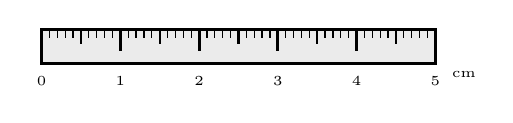
\begin{tikzpicture}[x=1cm, y=1cm, every node/.style={font=\scriptsize, text=black}]
      \draw[black, line width=1.1pt, fill=panelgray] (0,0) rectangle (5.0, 0.44);
      \foreach \m in {0,...,50}{
        \pgfmathsetmacro{\xval}{\m*0.1}
        \draw[black, line width=0.45pt] (\xval, 0.44) -- (\xval, 0.33);
      }
      \foreach \h in {0,0.5,...,5.0}{
        \draw[black, line width=0.8pt] (\h, 0.44) -- (\h, 0.25);
      }
      \foreach \c in {0,1,2,3,4,5}{
        \draw[black, line width=1.1pt] (\c, 0.44) -- (\c, 0.16);
        \node[below=1pt, font=\tiny] at (\c, 0.0) {\en{\c}};
      }
      \node[right=2pt, font=\tiny] at (5.02, -0.14) {\en{cm}};
    \end{tikzpicture}
  \end{tcolorbox}
\end{minipage}

\vspace{3.5pt}

% --- ផ្នែកទី ១៖ សកម្មភាព 1 — បន្ទះបត់ក្រដាស BC = 6.0 cm (ទ្រេត 12° បំបាត់ verticality bias, x=1cm, y=1cm) ---
\textbf{១. សកម្មភាព \en{1} ៖ បត់បន្ទះ $BC=6.0\unit{cm}$ ឱ្យ $B$ ត្រួតលើ $C$ រកផ្នត់មេដ្យាទ័រ $\Delta$ និងផ្ទៀង $M, N$ (\en{x=1cm, y=1cm})}

\vspace{2pt}
\noindent
\begin{minipage}[c]{8.85cm}
  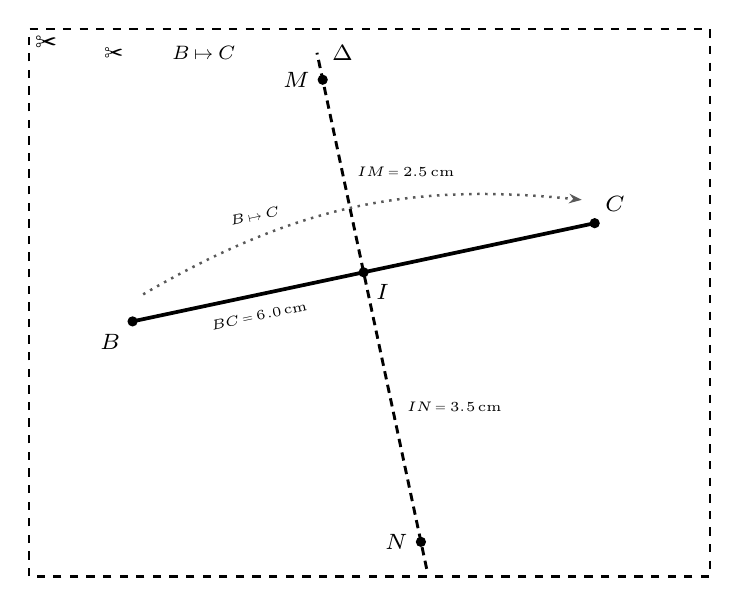
\begin{tikzpicture}[x=1cm, y=1cm, every node/.style={font=\scriptsize, text=black}]
    % Cuttable box: 8.65 cm x 6.95 cm
    \draw[black, dashed, line width=0.95pt] (0, 0) rectangle (8.65, 6.95);
    \node[anchor=north west, inner sep=1pt, font=\footnotesize] at (0.04, 6.91) {\scissors};
    \node[anchor=north west, font=\scriptsize] at (0.45, 6.86) {\textbf{កាត់ \scissors{} រួចបត់ $B \mapsto C$}};

    % Exact 1:1 tilted 12 deg segment BC = 6.0 cm centered at I = (4.25, 3.86)
    % cos(12)=0.9781476, sin(12)=0.2079117
    % B = (4.25 - 2.93444, 3.86 - 0.623735) = (1.3156, 3.2363)
    % C = (4.25 + 2.93444, 3.86 + 0.623735) = (7.1844, 4.4837)
    % M (+2.5 cm along normal (-0.2079117, 0.9781476)) = (3.7302, 6.3054)
    % N (-3.5 cm along normal) = (4.9777, 0.4365)
    \coordinate (I) at (4.25, 3.86);
    \coordinate (B) at (1.3156, 3.2363);
    \coordinate (C) at (7.1844, 4.4837);
    \coordinate (M) at (3.7302, 6.3054);
    \coordinate (N) at (4.9777, 0.4365);
    \coordinate (Dtop) at (3.6574, 6.6477);
    \coordinate (Dbot) at (5.0505, 0.0942);

    % Dashed crease guide Delta & solid BC
    \draw[black, densely dashed, line width=1.05pt] (Dbot) -- (Dtop);
    \draw[black, line width=1.35pt] (B) -- (C);
    % Light fold curve hint B -> C
    \draw[darkline, dotted, line width=0.9pt, -{Stealth[length=1.6mm]}] (1.45, 3.58) to[bend left=18] (7.02, 4.78);
    \node[font=\tiny, rotate=12] at (2.75, 4.55) {បត់ $B\mapsto C$};

    % Points & clear labels
    \fill[black] (B) circle (0.065) node[below left=1pt, font=\footnotesize] {$B$};
    \fill[black] (C) circle (0.065) node[above right=0.5pt, font=\footnotesize] {$C$};
    \fill[black] (I) circle (0.065) node[below right=1pt, font=\footnotesize] {$I$};
    \fill[black] (M) circle (0.065) node[left=2pt, font=\footnotesize] {$M$};
    \fill[black] (N) circle (0.065) node[left=2pt, font=\footnotesize] {$N$};
    \node[right=2pt, font=\footnotesize] at (Dtop) {$\Delta$};
    \node[font=\tiny, rotate=12] at ($(B)!0.26!(C)+(0.08,-0.25)$) {$BC = 6.0\unit{cm}$};
    \node[font=\tiny, right=2pt] at ($(I)!0.52!(M)$) {$IM = 2.5\unit{cm}$};
    \node[font=\tiny, right=2pt] at ($(I)!0.50!(N)$) {$IN = 3.5\unit{cm}$};
  \end{tikzpicture}
\end{minipage}%
\hfill
\begin{minipage}[c]{9.85cm}
  \begin{tcolorbox}[
    enhanced, sharp corners, colback=white, colframe=black,
    boxrule=1.0pt, boxsep=1pt, top=3.5pt, bottom=3.5pt, left=5pt, right=5pt,
    title={\textbf{កំណត់ត្រាសកម្មភាព \en{1} ៖ បត់រកសោភ្លោះ \en{\&} វាស់ $M, N$}},
    colbacktitle=headgray, coltitle=black, fonttitle=\fontsize{8.1pt}{11pt}\selectfont
  ]
    \raggedright\fontsize{7.85pt}{11.2pt}\selectfont
    \textbf{ជំហាន ១ (បត់ក្រដាស)៖} បត់បន្ទះឱ្យ $B$ ត្រួតលើ $C$ ច្បាស់តាមផ្នត់ $\Delta$~។\\[2pt]
    \textbf{ជំហាន ២ (វាស់សោភ្លោះ ២ យ៉ាង)៖}\\[1.5pt]
    \renewcommand{\arraystretch}{1.12}
    \begin{tabular}{|L{3.45cm}|L{3.65cm}|L{1.15cm}|}
      \hline
      \cellcolor{panelgray}\textbf{ធាតុវាស់លើផ្នត់ $\Delta$} & \cellcolor{panelgray}\textbf{រង្វាស់ខ្នាត \en{1:1} ជាក់ស្ដែង} & \cellcolor{panelgray}\textbf{សន្និដ្ឋាន} \\ \hline
      ១. ចំណុច $I$ លើ $BC$ & $IB=\underline{\hspace{0.55cm}}\unit{cm},\; IC=\underline{\hspace{0.55cm}}\unit{cm}$ & \chkbox\ $=3.0$ \\ \hline
      ២. មុំត្រង់ $I$ & $\ang{MIB}=\underline{\hspace{0.48cm}}^\circ,\; \ang{MIC}=\underline{\hspace{0.48cm}}^\circ$ & \chkbox\ $=90^\circ$ \\ \hline
      ៣. ពី $M$ ($2.5\unit{cm}$ លើ $I$) & $MB=\underline{\hspace{0.55cm}}\unit{cm},\; MC=\underline{\hspace{0.55cm}}\unit{cm}$ & \chkbox\ $MB=MC$ \\ \hline
      ៤. ពី $N$ ($3.5\unit{cm}$ ក្រោម $I$) & $NB=\underline{\hspace{0.55cm}}\unit{cm},\; NC=\underline{\hspace{0.55cm}}\unit{cm}$ & \chkbox\ $NB=NC$ \\ \hline
    \end{tabular}\\[3pt]
    \textbf{សង្កេតរកឃើញ៖} ផ្នត់ $\Delta$ កាត់តាម\textbf{ចំណុចកណ្ដាល $I$} ($IB=IC=3\unit{cm}$) ផង និង\textbf{កែង $90^\circ$} នឹង $BC$ ផង $\implies$ គ្រប់ចំណុចលើ $\Delta$ ($M, N$) សុទ្ធតែ\textbf{ស្មើចម្ងាយពី $B, C$}!
  \end{tcolorbox}
\end{minipage}

\vspace{3.5pt}

% --- ផ្នែកទី ២៖ សកម្មភាព 2 (Dual POE: POE 2A សោម្ខាង & POE 2B ដែកឈាន ២ ចំណុច) ---
\textbf{២. សកម្មភាព \en{2} (\en{Dual POE}) ៖ \en{POE 2A} (សាកសោតែម្ខាង) \en{\&} \en{POE 2B} (ធ្នូដែកឈានប្រសព្វ ២ ចំណុច) (\en{x=1cm, y=1cm})}

\vspace{2pt}
% --- POE 2A: Panel X (60° median) & Panel Y (off-center perp) side by side ---
\noindent
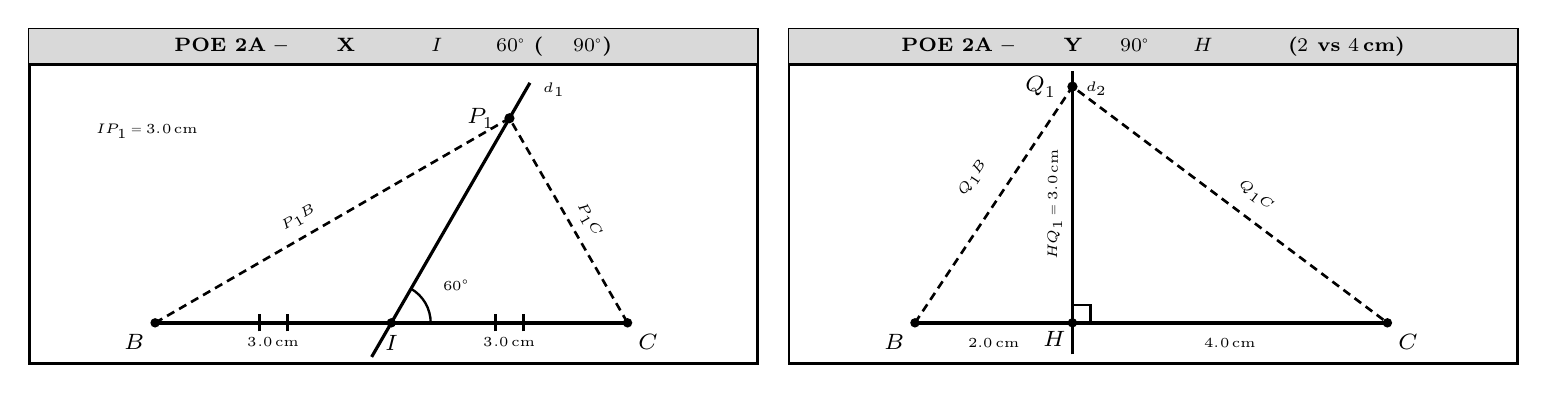
\begin{tikzpicture}[x=1cm, y=1cm, every node/.style={font=\scriptsize, text=black}]
  % === Panel X: BC=6.0 cm, slanted median d1 through I at 60 deg, P1 at 3.0 cm from I ===
  \begin{scope}[shift={(0,0)}]
    \draw[black, line width=1.05pt] (0, 0) rectangle (9.25, 4.25);
    \fill[headgray] (0, 3.80) rectangle (9.25, 4.25);
    \draw[black, line width=0.85pt] (0, 3.80) -- (9.25, 3.80);
    \node[font=\scriptsize] at (4.625, 4.025) {\textbf{\en{POE 2A} -- ផ្ទាំង \en{X}៖ កាត់កណ្ដាល $I$ តែទ្រេត $60^\circ$ (ខ្វះ $90^\circ$)}};

    % Exact 1:1 coords: B=(1.60,0.52), C=(7.60,0.52), I=(4.60,0.52), P1=(6.10, 3.1181)
    \coordinate (XB) at (1.60, 0.52);
    \coordinate (XC) at (7.60, 0.52);
    \coordinate (XI) at (4.60, 0.52);
    \coordinate (XP1) at (6.10, 3.1181);
    \draw[black, line width=1.25pt, tk2] (XB) -- (XI);
    \draw[black, line width=1.25pt, tk2] (XI) -- (XC);
    \draw[black, line width=1.15pt] (4.35, 0.087) -- (6.36, 3.568);
    \draw[black, densely dashed, line width=0.95pt] (XB) -- (XP1) -- (XC);
    \pic[draw=black, line width=0.85pt, angle radius=5.0mm]{angle=XC--XI--XP1};
    \node[font=\tiny] at ($(XI)+(30:0.95)$) {$60^\circ$};
    \fill[black] (XB) circle (0.06) node[below left=0.5pt, font=\footnotesize] {$B$};
    \fill[black] (XC) circle (0.06) node[below right=0.5pt, font=\footnotesize] {$C$};
    \fill[black] (XI) circle (0.06) node[below=1pt, font=\footnotesize] {$I$};
    \fill[black] (XP1) circle (0.065) node[left=2pt, font=\footnotesize] {$P_1$};
    \node[right=1.5pt, font=\tiny] at (6.36, 3.48) {$d_1$};
    \node[below=1pt, font=\tiny] at (3.10, 0.50) {$3.0\unit{cm}$};
    \node[below=1pt, font=\tiny] at (6.10, 0.50) {$3.0\unit{cm}$};
    \node[font=\tiny, rotate=30] at ($(XB)!0.42!(XP1)+(-0.18,0.16)$) {វាស់ $P_1B$};
    \node[font=\tiny, rotate=-60] at ($(XC)!0.52!(XP1)+(0.22,0.08)$) {វាស់ $P_1C$};
    \node[font=\tiny] at (1.50, 2.95) {$IP_1=3.0\unit{cm}$};
  \end{scope}

  % === Panel Y: BC=6.0 cm, off-center perp d2 at H (HB=2.0, HC=4.0), Q1 at 3.0 cm from H ===
  \begin{scope}[shift={(9.65,0)}]
    \draw[black, line width=1.05pt] (0, 0) rectangle (9.25, 4.25);
    \fill[headgray] (0, 3.80) rectangle (9.25, 4.25);
    \draw[black, line width=0.85pt] (0, 3.80) -- (9.25, 3.80);
    \node[font=\scriptsize] at (4.625, 4.025) {\textbf{\en{POE 2A} -- ផ្ទាំង \en{Y}៖ កែង $90^\circ$ ត្រង់ $H$ តែខុសកណ្ដាល ($2$ \en{vs} $4\unit{cm}$)}};

    % Exact 1:1 coords: B=(1.60,0.52), C=(7.60,0.52), H=(3.60,0.52), Q1=(3.60, 3.52)
    \coordinate (YB) at (1.60, 0.52);
    \coordinate (YC) at (7.60, 0.52);
    \coordinate (YH) at (3.60, 0.52);
    \coordinate (YQ1) at (3.60, 3.52);
    \draw[black, line width=1.25pt] (YB) -- (YC);
    \draw[black, line width=1.15pt] (3.60, 0.12) -- (3.60, 3.72);
    \draw[black, densely dashed, line width=0.95pt] (YB) -- (YQ1) -- (YC);
    \pic[draw=black, line width=0.85pt, angle radius=2.3mm]{right angle=YC--YH--YQ1};
    \fill[black] (YB) circle (0.06) node[below left=0.5pt, font=\footnotesize] {$B$};
    \fill[black] (YC) circle (0.06) node[below right=0.5pt, font=\footnotesize] {$C$};
    \fill[black] (YH) circle (0.06);
    \node[fill=white, inner sep=0.6pt, font=\footnotesize] at ($(YH)+(-0.24, -0.20)$) {$H$};
    \fill[black] (YQ1) circle (0.065) node[left=2.5pt, font=\footnotesize] {$Q_1$};
    \node[below right=1pt, font=\tiny] at (3.62, 3.74) {$d_2$};
    \node[below=1.5pt, font=\tiny] at (2.60, 0.50) {$2.0\unit{cm}$};
    \node[below=1.5pt, font=\tiny] at (5.60, 0.50) {$4.0\unit{cm}$};
    \node[font=\tiny, rotate=90] at (3.38, 2.02) {$HQ_1=3.0\unit{cm}$};
    \node[font=\tiny, rotate=56] at ($(YB)!0.50!(YQ1)+(-0.34,0.22)$) {វាស់ $Q_1B$};
    \node[font=\tiny, rotate=-37] at ($(YC)!0.50!(YQ1)+(0.22,0.20)$) {វាស់ $Q_1C$};
  \end{scope}
\end{tikzpicture}

\vspace{2pt}
\begin{tcolorbox}[
  enhanced, sharp corners, colback=panelgray, colframe=black,
  boxrule=0.85pt, boxsep=1pt, top=2.5pt, bottom=2.5pt, left=5pt, right=5pt
]
  \raggedright\fontsize{7.8pt}{10.9pt}\selectfont
  \textbf{\en{POE 2A} (ទស្សន៍ទាយ--វាស់--ពន្យល់)៖}
  \textbf{P:} តើ $P_1B=P_1C$ និង $Q_1B=Q_1C$ ទេ? \chkbox\ ស្មើ \chkbox\ មិនស្មើ \quad
  \textbf{O:} ផ្ទាំង X៖ $P_1B=\underline{\hspace{0.55cm}}\unit{cm},\; P_1C=\underline{\hspace{0.55cm}}\unit{cm}$ \en{|} ផ្ទាំង Y៖ $Q_1B=\underline{\hspace{0.55cm}}\unit{cm},\; Q_1C=\underline{\hspace{0.55cm}}\unit{cm}$\\
  \textbf{E:} ហេតុអ្វីជាប់សោតែ ១ ម្ខាង (X ខ្វះ $90^\circ$, Y ខ្វះ $IB=IC$) ធ្វើឱ្យ $P_1, Q_1$ មិនស្មើចម្ងាយពី $B, C$? $\underline{\hspace{6.2cm}}$
\end{tcolorbox}

\vspace{3pt}

% --- POE 2B: Dual-Arc Compass Locus (BC = 6.0 cm, r = 4.5 cm) x=1cm, y=1cm ---
\noindent
\begin{minipage}[c]{9.45cm}
  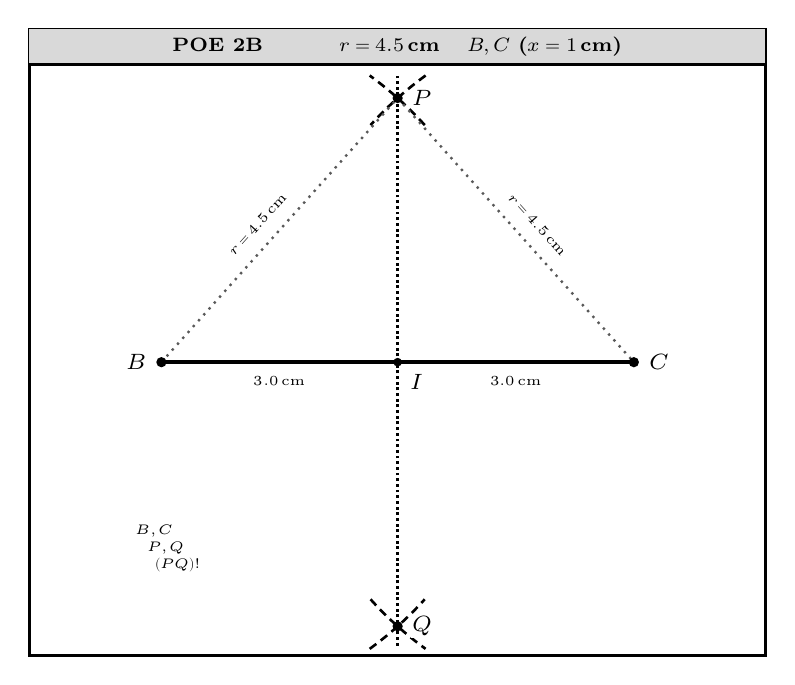
\begin{tikzpicture}[x=1cm, y=1cm, every node/.style={font=\scriptsize, text=black}]
    % Box: 9.35 cm x 7.95 cm
    \draw[black, line width=1.05pt, fill=white] (0, 0) rectangle (9.35, 7.95);
    \fill[headgray] (0, 7.50) rectangle (9.35, 7.95);
    \draw[black, line width=0.85pt] (0, 7.50) -- (9.35, 7.50);
    \node[font=\scriptsize] at (4.675, 7.725) {\textbf{\en{POE 2B}៖ ធ្នូដែកឈាន $r=4.5\unit{cm}$ ពី $B, C$ ($x=1\unit{cm}$)}};

    % Exact 1:1 coords: B=(1.68, 3.72), C=(7.68, 3.72) -> BC = 6.000 cm
    % Midpoint I=(4.68, 3.72), h = sqrt(4.5^2 - 3.0^2) = 3.3541 cm
    % P=(4.68, 7.0741), Q=(4.68, 0.3659)
    \coordinate (B) at (1.68, 3.72);
    \coordinate (C) at (7.68, 3.72);
    \coordinate (I) at (4.68, 3.72);
    \coordinate (P) at (4.68, 7.0741);
    \coordinate (Q) at (4.68, 0.3659);

    % Main segment BC (solid 1.35pt)
    \draw[black, line width=1.35pt] (B) -- (C);
    % Straightedge line (PQ) guide (densely dotted)
    \draw[black, densely dotted, line width=1.05pt] (4.68, 0.12) -- (4.68, 7.36);
    % Dual-arc compass target guides r = 4.5 cm from B and C (sweeping +/- 6 deg around P, Q)
    \draw[black, densely dashed, line width=0.95pt] ($(B)+(42:4.5)$) arc (42:54:4.5);
    \draw[black, densely dashed, line width=0.95pt] ($(B)+(-54:4.5)$) arc (-54:-42:4.5);
    \draw[black, densely dashed, line width=0.95pt] ($(C)+(126:4.5)$) arc (126:138:4.5);
    \draw[black, densely dashed, line width=0.95pt] ($(C)+(-138:4.5)$) arc (-138:-126:4.5);
    % Faint compass radii guides to P
    \draw[darkline, dotted, line width=0.85pt] (B) -- (P) -- (C);

    \fill[black] (B) circle (0.065) node[left=2pt, font=\footnotesize] {$B$};
    \fill[black] (C) circle (0.065) node[right=2pt, font=\footnotesize] {$C$};
    \fill[black] (I) circle (0.055) node[below right=1pt, font=\footnotesize] {$I$};
    \fill[black] (P) circle (0.065) node[right=4.5pt, fill=white, inner sep=0.6pt, font=\footnotesize] {$P$};
    \fill[black] (Q) circle (0.065) node[right=4.5pt, fill=white, inner sep=0.6pt, font=\footnotesize] {$Q$};
    \node[below=1pt, font=\tiny] at (3.18, 3.70) {$3.0\unit{cm}$};
    \node[below=1pt, font=\tiny] at (6.18, 3.70) {$3.0\unit{cm}$};
    \node[font=\tiny, rotate=48] at ($(B)!0.48!(P)+(-0.22,0.14)$) {$r=4.5\unit{cm}$};
    \node[font=\tiny, rotate=-48] at ($(C)!0.48!(P)+(0.22,0.14)$) {$r=4.5\unit{cm}$};
    \node[font=\tiny, align=left] at (1.50, 1.40) {កំណត់សម្គាល់៖\\គូសធ្នូពី $B, C$\\ប្រសព្វត្រង់ $P, Q$\\រួចដាក់បន្ទាត់ $(PQ)$!};
  \end{tikzpicture}
\end{minipage}%
\hfill
\begin{minipage}[c]{9.30cm}
  \begin{tcolorbox}[
    enhanced, sharp corners, colback=white, colframe=black,
    boxrule=1.0pt, boxsep=1pt, top=3.5pt, bottom=3.5pt, left=5pt, right=5pt,
    title={\textbf{កំណត់ត្រា \en{POE 2B} ៖ ធ្នូដែកឈាន $r=4.5\unit{cm}$ \& តារាងផ្ទៀង}},
    colbacktitle=headgray, coltitle=black, fonttitle=\fontsize{8.1pt}{11pt}\selectfont
  ]
    \raggedright\fontsize{7.8pt}{11.2pt}\selectfont
    \textbf{\en{P} -- ទស្សន៍ទាយ៖} បើបើកដែកឈាន $r=4.5\unit{cm}$ ($>3\unit{cm}$) ពី $B$ និង $C$ ប្រសព្វត្រង់ $P$ ខាងលើ និង $Q$ ខាងក្រោម តើបន្ទាត់ត្រង់ $(PQ)$ កាត់ $BC$ ត្រង់ណា និងមុំប៉ុន្មានដឺក្រេ?\\
    \chkbox\ កាត់ត្រង់កណ្ដាល $I$ មុំ $90^\circ$ \quad \chkbox\ កាត់ខុសកណ្ដាល\\[3pt]
    \textbf{\en{O} -- វាស់ផ្ទៀងខ្នាត \en{1:1} ក្រោយគូសបន្ទាត់ $(PQ)$៖}\\[2pt]
    \renewcommand{\arraystretch}{1.15}
    \begin{tabular}{|L{2.95cm}|L{3.65cm}|L{1.15cm}|}
      \hline
      \cellcolor{panelgray}\textbf{ធាតុត្រួតពិនិត្យ} & \cellcolor{panelgray}\textbf{រង្វាស់ជាក់ស្ដែង (\en{cm} / $^\circ$)} & \cellcolor{panelgray}\textbf{ផ្ទៀង} \\ \hline
      ១. កាំពី $B, C$ ទៅ $P$ & $PB=\underline{\hspace{0.55cm}},\; PC=\underline{\hspace{0.55cm}}$ & \chkbox\ $=4.5$ \\ \hline
      ២. កាំពី $B, C$ ទៅ $Q$ & $QB=\underline{\hspace{0.55cm}},\; QC=\underline{\hspace{0.55cm}}$ & \chkbox\ $=4.5$ \\ \hline
      ៣. ទីតាំង $I$ លើ $BC$ & $IB=\underline{\hspace{0.55cm}},\; IC=\underline{\hspace{0.55cm}}$ & \chkbox\ $=3.0$ \\ \hline
      ៤. មុំ $(PQ)$ និង $BC$ & $\ang{PIB}=\underline{\hspace{0.50cm}}^\circ$ & \chkbox\ $=90^\circ$ \\ \hline
    \end{tabular}\\[4pt]
    \textbf{\en{E} -- ពន្យល់៖} ១) ហេតុអ្វី $(PQ)$ ក្លាយជាមេដ្យាទ័រដោយមិនបាច់វាស់ $I$ ឬ $90^\circ$? ២) បើ $r \le 3\unit{cm}$ ហេតុអ្វីធ្នូមិនកាត់គ្នា?\\[3pt]
    \rule{\linewidth}{0.55pt}\\[10pt]
    \rule{\linewidth}{0.55pt}
  \end{tcolorbox}
\end{minipage}

\clearpage

% ============================================================================
% ទំព័រទី ២៖ E4 Elaborate — កាត "កាតសោភ្លោះ និងធ្នូប្រសព្វពីរចំណុច" (២ ប័ណ្ណ)
% ============================================================================
\pagebanner{សម្ភារៈទី ២៖ កាត \enbf{E4} «កាតសោភ្លោះ និងធ្នូប្រសព្វពីរចំណុច»}{ទំព័រ ២/៦ \en{-- E4 Elaborate} (កាត់ ២ ប័ណ្ណ \scissors)}

\newcommand{\eFourCardPB}[1]{%
\begin{tcolorbox}[
  enhanced, sharp corners, colback=white, colframe=white,
  borderline={1.0pt}{0pt}{black, dashed},
  boxsep=1pt, top=3.5pt, bottom=3.5pt, left=5pt, right=5pt
]
  \begin{tcolorbox}[
    enhanced, sharp corners, colback=headgray, colframe=black,
    boxrule=0.8pt, boxsep=1pt, top=2.5pt, bottom=2.5pt, left=5pt, right=5pt, after skip=4.5pt
  ]
    \fontsize{8.3pt}{11.2pt}\selectfont
    \textbf{\scissors\ កាតសកម្មភាព \en{E4} (#1) \en{--} កាតសោភ្លោះ និងធ្នូប្រសព្វពីរចំណុច} \hfill ក្រុម៖ $\underline{\hspace{2.8cm}}$
  \end{tcolorbox}

  \noindent
  \begin{minipage}[t]{7.45cm}
    \vspace{0pt}
    \fontsize{7.85pt}{11.0pt}\selectfont
    \textbf{លំហាត់គំរូ \en{E4} (រូបទំព័រ ១៥៦)៖} \textbf{(ក)} គេឱ្យ $I$ ជាចំណុចកណ្ដាលនៃ $BC$ និង $MB=MC$~។ បង្ហាញថា $(MI)$ ជាមេដ្យាទ័រនៃ $BC$ (ទ្រឹស្ដីបទច្រាស)~។ \textbf{(ខ)} បើ $N$ មាន $NB=NC$ បង្ហាញថា $(MN)\equiv\Delta$ ដោយមិនវាស់ $I$~។
    \begin{center}
    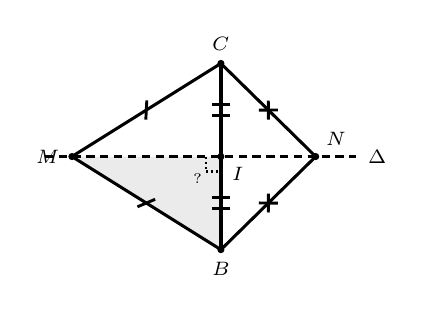
\begin{tikzpicture}[scale=0.86, every node/.style={font=\scriptsize, text=black}]
      % Book p. 156 vertical BC (C top, B bottom, I midpoint), horizontal Delta (M left, N right closer to I)
      \coordinate (B) at (2.55, 0.0);
      \coordinate (C) at (2.55, 2.75);
      \coordinate (I) at (2.55, 1.375);
      \coordinate (M) at (0.35, 1.375);
      \coordinate (N) at (3.95, 1.375);

      % Light monochrome shading on ∆MIB to trace ∆MIB vs ∆MIC cleanly
      \fill[panelgray] (M) -- (I) -- (B) -- cycle;
      % Vertical BC with '=' (tk2) on IC and IB
      \draw[black, line width=1.2pt, tk2] (C) -- (I);
      \draw[black, line width=1.2pt, tk2] (I) -- (B);
      % M-C, M-B with '/' (tkslash); N-C, N-B with 'x' (tkcross)
      \draw[black, line width=1.1pt, tkslash] (M) -- (C);
      \draw[black, line width=1.1pt, tkslash] (M) -- (B);
      \draw[black, line width=1.1pt, tkcross] (N) -- (C);
      \draw[black, line width=1.1pt, tkcross] (N) -- (B);
      % Dashed auxiliary line (MN) / Delta (NOT pre-marking 90° box since (ក) proves 90°!)
      \draw[black, densely dashed, line width=1.15pt] (-0.05, 1.375) -- (4.55, 1.375);
      % Small '?' at I angle to show students prove 90°
      \draw[black, densely dotted, line width=0.8pt] ($(I)+(-0.22,0)$) -- ($(I)+(-0.22,-0.22)$) -- ($(I)+(0,-0.22)$);
      \node[font=\tiny] at ($(I)+(-0.34,-0.32)$) {$?$};

      \fill[black] (C) circle (1.5pt) node[above=1pt] {$C$};
      \fill[black] (B) circle (1.5pt) node[below=1pt] {$B$};
      \fill[black] (I) circle (1.5pt) node[below right=0.5pt] {$I$};
      \fill[black] (M) circle (1.5pt) node[left=1.5pt] {$M$};
      \fill[black] (N) circle (1.5pt) node[above right=0.5pt] {$N$};
      \node[right=1pt] at (4.55, 1.375) {$\Delta$};
    \end{tikzpicture}
    \end{center}
    \begin{tcolorbox}[enhanced, sharp corners, colback=panelgray, colframe=black, boxrule=0.7pt, boxsep=1pt, top=2.5pt, bottom=2.5pt, left=4pt, right=4pt]
      \raggedright\fontsize{7.3pt}{10.2pt}\selectfont
      \textbf{ពិនិត្យក្រោយ (\en{EIA} ៣០ វិនាទី) \en{--} អន្ទាក់ ១ ចំណុច \en{vs} ២ ចំណុច៖}\\
      បើមានតែ \textbf{១ ចំណុច} $P$ ស្មើចម្ងាយ ($PB=PC$) តើកំណត់បន្ទាត់ $\Delta$ តែមួយបានទេ? \chkbox\ មិនបាន (បន្ទាត់ទ្រេតរាប់មិនអស់កាត់ $P$!) ត្រូវការ \textbf{២ ចំណុច ($M, N$)} ទើបកំណត់ $(MN)\equiv\Delta$!
    \end{tcolorbox}
  \end{minipage}\hfill
  \begin{minipage}[t]{10.35cm}
    \vspace{0pt}
    \begin{tcolorbox}[enhanced, sharp corners, colback=white, colframe=black, boxrule=0.85pt, boxsep=1pt, top=3pt, bottom=3pt, left=5pt, right=5pt]
      \raggedright\fontsize{7.75pt}{11.1pt}\selectfont
      \textbf{(ក) សម្រាយទ្រឹស្ដីបទច្រាស [\en{[tracing]} តភ្ជាប់ $MI \Rightarrow$ ជ.ជ.ជ (\en{SSS}) $\Rightarrow 90^\circ$]៖}\\
      \chkbox\ អូសម្រាមដៃ \en{[tracing]} $\tri{MIB}$ និង $\tri{MIC}$ (គូស \enbf{=} លើ $IB, IC$, \enbf{/} លើ $MB, MC$)\\
      ក្នុង $\tri{MIB}$ និង $\tri{MIC}$ មាន៖\\
      \en{1)} $IB = \underline{\hspace{0.65cm}}$ \hspace{0.2cm} (\cnum{1} $I$ ចំណុចកណ្ដាល $BC$)\\
      \en{2)} $MB = \underline{\hspace{0.65cm}}$ \hspace{0.2cm} (សម្មតិកម្ម / កាំធ្នូស្មើ)\\
      \en{3)} ជ្រុងរួម $IM = \underline{\hspace{0.65cm}}$ \hspace{0.2cm} (បន្ទាត់ជំនួយតភ្ជាប់ $M$ ទៅ $I$)\\
      ដូចនេះ $\tri{MIB} \cg \tri{\underline{\hspace{0.75cm}}}$ (\cnum{3} $\underline{\hspace{1.25cm}}$) $\Rightarrow \ang{MIB}=\ang{\underline{\hspace{0.75cm}}}$\\
      ដោយ $\ang{MIB}+\ang{MIC}=180^\circ$ (មុំបន្ថែម) $\Rightarrow \ang{MIB}=\ang{MIC}=\underline{\hspace{0.55cm}}^\circ$ (\cnum{2})\\
      $\Rightarrow (MI)$ កែងនឹង $BC$ ត្រង់ $I \Rightarrow (MI)$ ជាមេដ្យាទ័រនៃ $BC$ (\cnum{5})!
    \end{tcolorbox}
    \vspace{2.5pt}
    \begin{tcolorbox}[enhanced, sharp corners, colback=panelgray, colframe=black, boxrule=0.85pt, boxsep=1pt, top=3pt, bottom=3pt, left=5pt, right=5pt]
      \raggedright\fontsize{7.75pt}{11.1pt}\selectfont
      \textbf{(ខ) គោលការណ៍ ២ ចំណុចនៃដែកឈាន [$(MN)\equiv\Delta$ ដោយមិនវាស់ $I$]៖}\\
      $\bullet$ តាម \textbf{(ក)}៖ $MB=MC \Rightarrow M \in \underline{\hspace{0.45cm}}$ និង $NB=NC \Rightarrow N \in \underline{\hspace{0.45cm}}$ (\cnum{5} ទ្រឹស្ដីបទច្រាស)\\
      $\bullet$ តាម ២ ចំណុច $M, N$ គូសបានបន្ទាត់\textbf{តែមួយគត់} $\Rightarrow (MN) \equiv \Delta$!
    \end{tcolorbox}
    \vspace{2.5pt}
    \raggedright{\fontsize{6.9pt}{9.6pt}\selectfont
    \textbf{ធនាគារ \cnum{1}--\cnum{5}៖} \cnum{1} កណ្ដាល ($IB=IC$) \en{|} \cnum{2} កែង $90^\circ$ \en{|} \cnum{3} ជ.ម.ជ/ជ.ជ.ជ/អ.ជ \en{|} \cnum{4} ផ្ទាល់ \en{|} \cnum{5} ច្រាស\par}
  \end{minipage}
\end{tcolorbox}%
}

\eFourCardPB{ប័ណ្ណទី ១}

\vspace{6pt}
\noindent\scissors\ \dotfill\ \textbf{កាត់តាមស្នាមចុចចែកជា ២ ប័ណ្ណ (\en{Cut Along Dashed Line})} \dotfill\ \scissors
\vspace{6pt}

\eFourCardPB{ប័ណ្ណទី ២}

\clearpage

% ============================================================================
% ទំព័រទី ៣៖ E5 Evaluate — "គណៈកម្មការផ្ទៀងសោភ្លោះ ៣ តួនាទី" ប្រតិបត្តិ (២ សន្លឹក)
% ============================================================================
\pagebanner{សម្ភារៈទី ៣៖ «គណៈកម្មការផ្ទៀងសោភ្លោះ ៣ តួនាទី» \enbf{--} ប្រតិបត្តិ \enbf{(E5 \& E1)}}{ទំព័រ ៣/៦ \en{-- E5 Evaluate} (កាត់ ២ សន្លឹក \scissors)}

\newcommand{\eFiveSheetPB}[1]{%
\begin{tcolorbox}[
  enhanced, sharp corners, colback=white, colframe=white,
  borderline={1.0pt}{0pt}{black, dashed},
  boxsep=1pt, top=2pt, bottom=2pt, left=4.5pt, right=4.5pt
]
  \begin{tcolorbox}[
    enhanced, sharp corners, colback=headgray, colframe=black,
    boxrule=0.8pt, boxsep=1pt, top=1.5pt, bottom=1.5pt, left=4pt, right=4pt, after skip=2pt
  ]
    \fontsize{6.95pt}{9.2pt}\selectfont
    \textbf{\scissors\ គណៈកម្មការផ្ទៀងសោភ្លោះ (#1)} \en{|} ក្រុម៖ $\underline{\hspace{0.85cm}}$ \hfill \textbf{ប្រតិបត្តិ៖} $BC=8\unit{cm}$, $\Delta$ មេដ្យាទ័រ, $M\in\Delta$, $MB=3x-1$, $MC=x+7$, $NB=NC=6\unit{cm}$
  \end{tcolorbox}

  \renewcommand{\arraystretch}{1.01}
  {\centering\setlength{\tabcolsep}{3.5pt}%
  \begin{tabular}{|L{6.40cm}|L{5.85cm}|L{5.35cm}|}
    \hline
    \cellcolor{panelgray}\centering\arraybackslash\fontsize{7.3pt}{9.6pt}\selectfont\textbf{តួនាទី ១៖ គូសសញ្ញា \en{\&} ផ្ទៀងសោភ្លោះ}\newline {\fontsize{6.7pt}{8.7pt}\selectfont \textbf{\en{Pause-Ask!}} \en{--} សម្គាល់ $IB=IC$ \en{+} $90^\circ$ ត្រង់ $I$} &
    \cellcolor{panelgray}\centering\arraybackslash\fontsize{7.3pt}{9.6pt}\selectfont\textbf{តួនាទី ២៖ សម្រាយ \cnum{1}--\cnum{4} \en{\&} ពិជគណិត}\newline {\fontsize{6.7pt}{8.7pt}\selectfont រក $IB, IC$, សមីការ $x$ និង $MB=MC$} &
    \cellcolor{panelgray}\centering\arraybackslash\fontsize{7.3pt}{9.6pt}\selectfont\textbf{តួនាទី ៣៖ ច្រាស \cnum{5} \en{\&} បិទ \en{E1}}\newline {\fontsize{6.7pt}{8.7pt}\selectfont \textbf{\en{Pause-Review!}} $N\in\Delta \Rightarrow M,I,N$ រួមបន្ទាត់} \\ \hline

    % --- Column 1: Village Solar Water Station Diagram (tilted BC = 8 cm) ---
    {\centering
    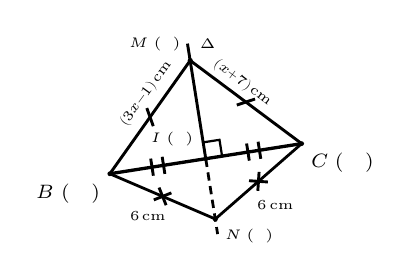
\begin{tikzpicture}[baseline={([yshift=-1ex]current bounding box.north)}, scale=0.58, every node/.style={font=\scriptsize, text=black}]
      % Tilted 9 deg BC: B=(-2.10, -0.33), C=(2.10, 0.33), I=(0,0)
      \coordinate (B) at (-2.10, -0.33);
      \coordinate (C) at (2.10, 0.33);
      \coordinate (I) at (0, 0);
      \coordinate (M) at (-0.34, 2.15);
      \coordinate (N) at (0.21, -1.32);
      \coordinate (Dtop) at (-0.40, 2.52);
      \coordinate (Dbot) at (0.26, -1.65);

      % Segment BC with '=' ticks (tk2)
      \draw[black, line width=1.2pt, tk2] (B) -- (I);
      \draw[black, line width=1.2pt, tk2] (I) -- (C);
      % Delta solid above I, dashed extension below I toward N
      \draw[black, line width=1.05pt] (I) -- (Dtop);
      \draw[black, densely dashed, line width=1.0pt] (I) -- (Dbot);
      \pic[draw=black, line width=0.8pt, angle radius=2.1mm]{right angle=C--I--M};

      % Pump cables MB, MC ('/') and Tank lines NB, NC ('x')
      \draw[black, line width=1.05pt, tkslash] (M) -- (B);
      \draw[black, line width=1.05pt, tkslash] (M) -- (C);
      \draw[black, line width=1.0pt, tkcross] (N) -- (B);
      \draw[black, line width=1.0pt, tkcross] (N) -- (C);

      \fill[black] (B) circle (1.5pt) node[below left=0pt] {$B$ (ភូមិ)};
      \fill[black] (C) circle (1.5pt) node[below right=0pt] {$C$ (ភូមិ)};
      \fill[black] (I) circle (1.5pt) node[above left=1pt, font=\tiny] {$I$ (លិច)};
      \fill[black] (M) circle (1.6pt) node[above left=0pt, font=\tiny] {$M$ (បូម)};
      \fill[black] (N) circle (1.6pt) node[below right=0pt, font=\tiny] {$N$ (អាង)};
      \node[right=1pt, font=\tiny] at (Dtop) {$\Delta$};

      \node[anchor=center, rotate=54, font=\tiny] at ($(B)!0.62!(M)+(-0.30, 0.22)$) {$(3x{-}1)\unit{cm}$};
      \node[anchor=center, rotate=-37, font=\tiny] at ($(C)!0.60!(M)+(0.18, 0.24)$) {$(x{+}7)\unit{cm}$};
      \node[below left=0pt, font=\tiny] at ($(B)!0.62!(N)$) {$6\unit{cm}$};
      \node[below right=0pt, font=\tiny] at ($(C)!0.62!(N)$) {$6\unit{cm}$};
    \end{tikzpicture}\par\vspace{1pt}
    {\fontsize{6.6pt}{8.5pt}\selectfont រូប៖ $BC=8\unit{cm}$, $\Delta$ មេដ្យាទ័រ ($M, N \in \Delta$)\par}}
    \fontsize{7.1pt}{9.7pt}\selectfont
    \chkbox\ គូស $90^\circ$ ត្រង់ $I$, \ticktwo\ លើ $IB, IC$, \tickslash\ លើ $MB, MC$, \tickcross\ លើ $NB, NC$\newline
    \chkbox\ \textbf{\en{Pause-Ask!}} «ហេតុអ្វី $IB=IC=4\unit{cm}$ និង $\Delta\perp BC$?»
    &
    % --- Column 2: (ក) ①–④ & Algebra x=4 -> MB=MC=11 cm ---
    \fontsize{7.3pt}{10.4pt}\selectfont
    \textbf{(ក) រក $IB, IC$, $x$ និង $MB=MC$៖}\par\vspace{2pt}
    $\bullet$ $I$ ចំណុចកណ្ដាល $BC=8\unit{cm}$ (\cnum{1}) $\Rightarrow IB=IC=\underline{\hspace{0.55cm}}\unit{cm}$\par\vspace{2pt}
    $\bullet$ $\Delta \perp BC$ ត្រង់ $I$ (\cnum{2}), $M \in \Delta \Rightarrow MB = \underline{\hspace{0.65cm}}$ (\cnum{4} ទ្រឹស្ដីផ្ទាល់)\par\vspace{2pt}
    $\bullet$ សមីការ៖ $3x - 1 = x + 7 \Rightarrow 2x = \underline{\hspace{0.50cm}} \Rightarrow x = \underline{\hspace{0.50cm}}$\newline
    $\Rightarrow MB = MC = 3(\underline{\hspace{0.40cm}})-1 = \underline{\hspace{0.55cm}}\unit{cm}$\par\vspace{4pt}
    \begin{tcolorbox}[enhanced, sharp corners, colback=panelgray, colframe=black, boxrule=0.65pt, boxsep=1pt, top=2.5pt, bottom=2.5pt, left=4.5pt, right=4.5pt]
      \raggedright\fontsize{6.9pt}{9.5pt}\selectfont
      \textbf{ធនាគារហេតុផល៖} \cnum{1} ចំណុចកណ្ដាល ($IB=IC$) \en{|} \cnum{2} មុំកែង $90^\circ$ \en{|} \cnum{4} ទ្រឹស្ដីផ្ទាល់ ($M\in\Delta\Rightarrow MB=MC$)
    \end{tcolorbox}
    &
    % --- Column 3: Pause-Review, (ខ) N∈Δ -> Collinear & E1 Closure ---
    \fontsize{7.2pt}{10.3pt}\selectfont
    \chkbox\ \textbf{\en{Pause-Review!}} ផ្ទៀង $x=4$៖ $3(4)-1=\underline{\hspace{0.45cm}},\; 4+7=\underline{\hspace{0.45cm}}\unit{cm}$!\par\vspace{3pt}
    \textbf{(ខ) ផ្ទៀងអាងទឹក $N$ (\cnum{5})៖}\newline
    ដោយ $NB = NC = 6\unit{cm} \Rightarrow N \in \underline{\hspace{0.50cm}}$ (\cnum{5} ទ្រឹស្ដីច្រាស)\newline
    $\Rightarrow$ ចំណុច $M, I, N$ \textbf{រួមបន្ទាត់ត្រង់ $\Delta$}!\par\vspace{4pt}
    \begin{tcolorbox}[enhanced, sharp corners, colback=panelgray, colframe=black, boxrule=0.7pt, boxsep=1pt, top=2.5pt, bottom=2.5pt, left=4.5pt, right=4.5pt]
      \raggedright\fontsize{6.85pt}{9.4pt}\selectfont
      \textbf{បិទបេសកកម្ម \en{E1} (ស្ថានីយបូមទឹកសូឡា)៖}\\
      ចំណុច $I$ នៅក្នុងប្រឡាយលិចទឹក ប៉ុន្តែទីទួលស្ងួតលើ $\Delta$ ($M$ ប្រវែង $11\unit{cm}$, អាង $N$ $6\unit{cm}$) រក្សាចម្ងាយស្មើពីភូមិ $B, C$ ១០០\%!
    \end{tcolorbox}
    \\ \hline
  \end{tabular}\par}
\end{tcolorbox}%
}

\eFiveSheetPB{សន្លឹកទី ១}

\vspace{3pt}
\noindent\scissors\ \dotfill\ \textbf{កាត់តាមស្នាមចុចចែកជា ២ សន្លឹក (\en{Cut Along Dashed Line})} \dotfill\ \scissors
\vspace{3pt}

\eFiveSheetPB{សន្លឹកទី ២}

\clearpage

% ============================================================================
% ទំព័រទី ៤៖ ផ្ទាំងយោងប្រចាំថ្នាក់រៀន — ទ្រឹស្ដីបទមេដ្យាទ័រនៃអង្កត់ & ធនាគារ ①–⑤
% ============================================================================
\begin{tcolorbox}[
  enhanced, sharp corners, colback=white, colframe=black,
  boxrule=1.5pt, borderline={0.6pt}{2.2pt}{black},
  boxsep=1pt, top=4pt, bottom=4pt, left=6pt, right=6pt
]
  \begin{center}
    {\muol\fontsize{11.4pt}{16pt}\selectfont ទ្រឹស្ដីបទមេដ្យាទ័រនៃអង្កត់ \enbf{(}ផ្ទាល់ \enbf{\&} ច្រាស\enbf{)} និងធនាគារ \cnum{1}\enbf{--}\cnum{5}}\\[1pt]
    {\fontsize{8.5pt}{11.8pt}\selectfont ផ្ទាំងយោងប្រចាំថ្នាក់រៀន (ស-ខ្មៅ) \en{--} មេរៀនទី១២ (២.១) លក្ខណៈមេដ្យាទ័រនៃអង្កត់ (សៀវភៅទំ.១៥៦)}\\[2pt]
    \khmflourish
  \end{center}
  \vspace{1pt}

  % --- ផ្នែកទី ១៖ រូបគោលទំ.១៥៦ + សម្រាយ ជ.ម.ជ (SAS) & ប្រអប់ទ្រឹស្ដីបទ (ផ្ទាល់ & ច្រាស) ---
  \noindent
  \begin{minipage}[t]{9.05cm}
    \begin{tcolorbox}[enhanced, sharp corners, colback=white, colframe=black, boxrule=0.95pt, boxsep=1pt, equal height group=posterTopPB, top=3pt, bottom=3pt, left=5pt, right=5pt]
      \textbf{\fontsize{7.9pt}{10.8pt}\selectfont រូបទំព័រ ១៥៦ \& សម្រាយបញ្ជាក់ផ្ទាល់ (ជ.ម.ជ / \en{SAS})៖}\\[2pt]
      \begin{minipage}[c]{3.75cm}
        \centering
        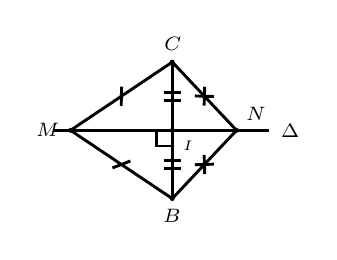
\begin{tikzpicture}[scale=0.68, every node/.style={font=\scriptsize, text=black}]
          % Book p. 156 vertical BC: C top, B bottom, '=' on IC, IB, 90 deg at I, horizontal Delta, M left (/), N right (x)
          \coordinate (B) at (2.15, 0.0);
          \coordinate (C) at (2.15, 2.55);
          \coordinate (I) at (2.15, 1.275);
          \coordinate (M) at (0.25, 1.275);
          \coordinate (N) at (3.35, 1.275);
          \draw[black, line width=1.15pt, tk2] (C) -- (I);
          \draw[black, line width=1.15pt, tk2] (I) -- (B);
          \draw[black, line width=1.05pt] (-0.05, 1.275) -- (3.95, 1.275);
          \draw[black, line width=1.05pt, tkslash] (M) -- (C);
          \draw[black, line width=1.05pt, tkslash] (M) -- (B);
          \draw[black, line width=1.05pt, tkcross] (N) -- (C);
          \draw[black, line width=1.05pt, tkcross] (N) -- (B);
          \pic[draw=black, line width=0.8pt, angle radius=2.0mm]{right angle=M--I--B};
          \fill[black] (C) circle (1.3pt) node[above=0.5pt] {$C$};
          \fill[black] (B) circle (1.3pt) node[below=0.5pt] {$B$};
          \fill[black] (I) circle (1.3pt) node[below right=0.5pt, font=\tiny] {$I$};
          \fill[black] (M) circle (1.3pt) node[left=1pt] {$M$};
          \fill[black] (N) circle (1.3pt) node[above right=0pt] {$N$};
          \node[right=1pt] at (3.95, 1.275) {$\Delta$};
        \end{tikzpicture}
      \end{minipage}\hfill
      \begin{minipage}[c]{4.80cm}
        \raggedright\fontsize{7.2pt}{10.2pt}\selectfont
        ក្នុង $\tri{MIB}$ និង $\tri{MIC}$ មាន៖\\
        $\bullet$ $IM$ ជាជ្រុងរួម\\
        $\bullet$ $\ang{MIB}=\ang{MIC}=90^\circ$ ($\Delta\perp BC$)\\
        $\bullet$ $IB=IC$ ($I$ កណ្ដាល $BC$)\\
        $\Rightarrow \tri{MIB}\cg\tri{MIC}$ (\textbf{លក្ខខណ្ឌ ជ.ម.ជ})\\
        \textbf{វិបាក៖} $MB=MC$, $\ang{IMB}=\ang{IMC}$, $\ang{IBM}=\ang{ICM}$~។
      \end{minipage}
    \end{tcolorbox}
  \end{minipage}\hfill
  \begin{minipage}[t]{8.75cm}
    \begin{tcolorbox}[enhanced, sharp corners, colback=panelgray, colframe=black, boxrule=0.95pt, boxsep=1pt, equal height group=posterTopPB, top=3pt, bottom=3pt, left=5pt, right=5pt]
      \raggedright\fontsize{7.4pt}{10.6pt}\selectfont
      \textbf{ប្រអប់ទ្រឹស្ដីបទ (ទំព័រ ១៥៦ \en{--} កែសម្រួលត្រឹមត្រូវ)៖}\\
      $\bullet$ \textbf{ទ្រឹស្ដីបទផ្ទាល់៖} គ្រប់ចំណុច\textbf{ស្ថិតនៅ}លើមេដ្យាទ័រនៃអង្កត់មួយត្រូវ\textbf{ស្ថិតនៅ}ស្មើចម្ងាយពីចុងទាំងពីរនៃអង្កត់នោះ\textbf{។} \textit{(បន្ថែម «។» និងឯកភាព «ស្ថិតនៅ»!)}\\
      $\bullet$ \textbf{ទ្រឹស្ដីបទច្រាស៖} គ្រប់ចំណុចដែល\textbf{ស្ថិតនៅ}ស្មើចម្ងាយពីចុងទាំងពីរនៃអង្កត់មួយ ចំណុចទាំងនេះគឺ\textbf{ស្ថិតនៅ}លើមេដ្យាទ័រនៃអង្កត់នោះ~។\\[2pt]
      \textbf{ក្បួនសោភ្លោះ (\en{Dual-Lock}):} ត្រូវមានទាំង \textbf{$IB=IC$} \textbf{និង} \textbf{$90^\circ$ ($\Delta\perp BC$)}!
    \end{tcolorbox}
  \end{minipage}

  \vspace{3.5pt}

  % --- ផ្នែកទី ២៖ តារាងធនាគារអំណះអំណាង ①–⑤ (លក្ខណៈមេដ្យាទ័រនៃអង្កត់) ---
  \fontsize{7.6pt}{10.6pt}\selectfont
  \renewcommand{\arraystretch}{1.05}
  \begin{tabular}{|C{0.70cm}|L{4.25cm}|L{6.30cm}|C{4.95cm}|}
    \hline
    \cellcolor{headgray}\textbf{លេខ} &
    \cellcolor{headgray}\centering\arraybackslash\textbf{ឈ្មោះអំណះអំណាង} &
    \cellcolor{headgray}\centering\arraybackslash\textbf{និមិត្តសញ្ញា និងរបៀបប្រើ} &
    \cellcolor{headgray}\centering\arraybackslash\textbf{រូបសម្គាល់ ស-ខ្មៅ} \\ \hline

    \cnum{1} &
    \textbf{ចំណុចកណ្ដាល ($IB=IC$)} &
    $I$ ជាចំណុចកណ្ដាលនៃអង្កត់ $BC \Rightarrow IB=IC$ ($=\tfrac{1}{2}BC$)~។ &
    \raisebox{-0.35\height}{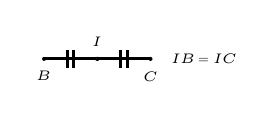
\begin{tikzpicture}[scale=0.52, every node/.style={font=\tiny, text=black}]
      \coordinate (b) at (0,0); \coordinate (i) at (1.3,0); \coordinate (c) at (2.6,0);
      \draw[black, line width=1.1pt, tk2] (b)--(i);
      \draw[black, line width=1.1pt, tk2] (i)--(c);
      \fill[black] (b) circle (1.4pt) node[below=1pt] {$B$};
      \fill[black] (i) circle (1.5pt) node[above=1pt] {$I$};
      \fill[black] (c) circle (1.4pt) node[below=1pt] {$C$};
      \node[right=2pt] at (2.75,0) {$IB=IC$};
    \end{tikzpicture}} \\ \hline

    \cnum{2} &
    \textbf{មុំកែង / បន្ទាត់កែង}\newline ($90^\circ, \Delta\perp BC$) &
    $\Delta\perp BC$ ត្រង់ $I \Rightarrow \ang{MIB}=\ang{MIC}=90^\circ$; ឬ $\ang{MIB}+\ang{MIC}=180^\circ \Rightarrow 90^\circ$~។ &
    \raisebox{-0.35\height}{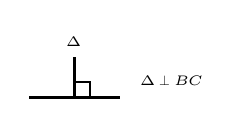
\begin{tikzpicture}[scale=0.50, every node/.style={font=\tiny, text=black}]
      \coordinate (b) at (0,0); \coordinate (i) at (1.15,0); \coordinate (c) at (2.3,0); \coordinate (m) at (1.15,1.05);
      \draw[black, line width=1.05pt] (b)--(c); \draw[black, line width=1.05pt] (i)--(m);
      \pic[draw=black, line width=0.8pt, angle radius=2.0mm]{right angle=c--i--m};
      \node[above=0pt] at (m) {$\Delta$}; \node[right=2pt] at (2.45,0.45) {$\Delta\perp BC$};
    \end{tikzpicture}} \\ \hline

    \cnum{3} &
    \textbf{លក្ខខណ្ឌ ជ.ម.ជ / ជ.ជ.ជ / អ.ជ} &
    ប្រើផ្ទាល់ ($\tri{MIB}\cg\tri{MIC}$ តាម ជ.ម.ជ) និងច្រាស (តាម ជ.ជ.ជ / អ.ជ)~។ &
    \raisebox{-0.35\height}{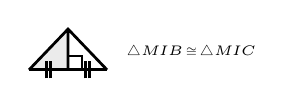
\begin{tikzpicture}[scale=0.45, every node/.style={font=\tiny, text=black}]
      \coordinate (b) at (0,0); \coordinate (i) at (1.1,0); \coordinate (m) at (1.1,1.15); \coordinate (c) at (2.2,0);
      \fill[panelgray] (b)--(i)--(m)--cycle;
      \draw[black, line width=1.0pt, tk2] (b)--(i); \draw[black, line width=1.0pt, tk2] (i)--(c);
      \draw[black, line width=1.0pt] (i)--(m) (b)--(m)--(c);
      \pic[draw=black, line width=0.75pt, angle radius=1.8mm]{right angle=c--i--m};
      \node[right=2pt] at (2.35,0.55) {$\tri{MIB}\cg\tri{MIC}$};
    \end{tikzpicture}} \\ \hline

    \cnum{4} &
    \textbf{និយមន័យនិងទ្រឹស្ដីបទផ្ទាល់}\newline ($M\in\Delta\Rightarrow MB=MC$) &
    $M$ ស្ថិតនៅលើមេដ្យាទ័រ $\Delta$ នៃ $BC \Rightarrow MB=MC$ និង $\ang{IMB}=\ang{IMC}$~។ &
    \raisebox{-0.35\height}{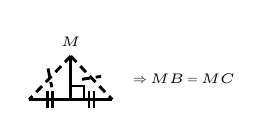
\begin{tikzpicture}[scale=0.48, every node/.style={font=\tiny, text=black}]
      \coordinate (b) at (0,0); \coordinate (i) at (1.1,0); \coordinate (c) at (2.2,0); \coordinate (m) at (1.1,1.15);
      \draw[black, line width=1.0pt, tk2] (b)--(i); \draw[black, line width=1.0pt, tk2] (i)--(c);
      \draw[black, line width=1.0pt] (i)--(m);
      \draw[black, densely dashed, line width=1.05pt, tkslash] (m)--(b);
      \draw[black, densely dashed, line width=1.05pt, tkslash] (m)--(c);
      \pic[draw=black, line width=0.75pt, angle radius=1.7mm]{right angle=c--i--m};
      \node[above=0pt] at (m) {$M$}; \node[right=2pt] at (2.35,0.55) {$\Rightarrow MB=MC$};
    \end{tikzpicture}} \\ \hline

    \cnum{5} &
    \textbf{ទ្រឹស្ដីបទច្រាស}\newline ($MB=MC\Rightarrow M\in\Delta, (MN)\equiv\Delta$) &
    ចំណុចស្មើចម្ងាយ $MB=MC \Rightarrow M\in\Delta$; ពីរចំណុច $M, N \Rightarrow (MN)\equiv\Delta$~។ &
    \raisebox{-0.35\height}{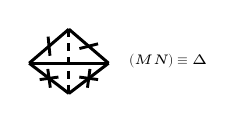
\begin{tikzpicture}[scale=0.48, every node/.style={font=\tiny, text=black}]
      \coordinate (b) at (0,0); \coordinate (c) at (2.1,0); \coordinate (m) at (1.05,0.90); \coordinate (n) at (1.05,-0.80);
      \draw[black, line width=1.0pt] (b)--(c);
      \draw[black, line width=1.1pt, tkslash] (m)--(b); \draw[black, line width=1.1pt, tkslash] (m)--(c);
      \draw[black, line width=1.1pt, tkcross] (n)--(b); \draw[black, line width=1.1pt, tkcross] (n)--(c);
      \draw[black, densely dashed, line width=1.1pt] (m)--(n);
      \node[right=2pt] at (2.25,0.05) {$(MN)\equiv\Delta$};
    \end{tikzpicture}} \\ \hline
  \end{tabular}

  \vspace{3.5pt}

  % --- ផ្នែកទី ៣៖ ប្រអប់ប្រៀបធៀប "ពុះមុំ vs មេដ្យាទ័រ" & "អន្ទាក់សោម្ខាង និង ១ ចំណុច" ---
  \noindent
  \begin{minipage}[t]{8.75cm}
    \begin{tcolorbox}[
      enhanced, sharp corners, colback=white, colframe=black,
      boxrule=1.1pt, boxsep=1pt, equal height group=posterBotPB,
      top=3pt, bottom=3pt, left=5pt, right=5pt,
      title={\textbf{ប្រៀបធៀបសំណុំចំណុច៖ ពុះមុំ \en{vs} មេដ្យាទ័រ}},
      colbacktitle=headgray, coltitle=black, fonttitle=\fontsize{8.0pt}{11pt}\selectfont
    ]
      \centering
      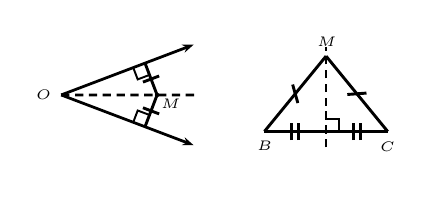
\begin{tikzpicture}[scale=0.58, every node/.style={font=\scriptsize, text=black}]
        % Left: Angle Bisector (equidistant from 2 sides via perpendiculars)
        \begin{scope}[shift={(0,0)}]
          \coordinate (O) at (0,1.0); \coordinate (X) at (2.9,2.1); \coordinate (Y) at (2.9,-0.1);
          \coordinate (M) at (2.1,1.0); \coordinate (A) at ($(O)!(M)!(X)$); \coordinate (B) at ($(O)!(M)!(Y)$);
          \draw[black, line width=1.0pt, -{Stealth[length=1.4mm]}] (O)--(X);
          \draw[black, line width=1.0pt, -{Stealth[length=1.4mm]}] (O)--(Y);
          \draw[black, densely dashed, line width=0.95pt] (O)--(3.0,1.0);
          \draw[black, line width=1.05pt, tk1] (M)--(A); \draw[black, line width=1.05pt, tk1] (M)--(B);
          \pic[draw=black, line width=0.7pt, angle radius=1.6mm]{right angle=M--A--O};
          \pic[draw=black, line width=0.7pt, angle radius=1.6mm]{right angle=M--B--O};
          \fill[black] (M) circle (1.4pt);
          \node[left=0pt, font=\tiny] at (O) {$O$}; \node[below right=1pt, font=\tiny, fill=white, inner sep=0.4pt] at (M) {$M$};
          \node[font=\tiny] at (1.5,-0.55) {\textbf{ពុះមុំ៖} កែងទៅ \textbf{ជ្រុង ២}};
        \end{scope}
        % Right: Perpendicular Bisector (equidistant from 2 endpoints)
        \begin{scope}[shift={(4.45,0.20)}]
          \coordinate (B) at (0,0); \coordinate (C) at (2.7,0); \coordinate (I) at (1.35,0); \coordinate (M) at (1.35,1.65);
          \draw[black, line width=1.0pt, tk2] (B)--(I); \draw[black, line width=1.0pt, tk2] (I)--(C);
          \draw[black, densely dashed, line width=0.95pt] (1.35,-0.35)--(1.35,1.85);
          \draw[black, line width=1.05pt, tkslash] (M)--(B); \draw[black, line width=1.05pt, tkslash] (M)--(C);
          \pic[draw=black, line width=0.7pt, angle radius=1.6mm]{right angle=C--I--M};
          \node[below=0pt, font=\tiny] at (B) {$B$}; \node[below=0pt, font=\tiny] at (C) {$C$}; \node[above=0pt, font=\tiny] at (M) {$M$};
          \node[font=\tiny] at (1.35,-0.75) {\textbf{មេដ្យាទ័រ៖} ត្រង់ទៅ \textbf{ចុង ២}};
        \end{scope}
      \end{tikzpicture}
      \par\vspace{1.5pt}\fontsize{7.4pt}{10.4pt}\selectfont
      $\bullet$ \textbf{ពុះមុំ៖} ស្មើចម្ងាយ\textbf{កែងទៅជ្រុង ២} ($MA\perp OX, MB\perp OY$)~។\\
      $\bullet$ \textbf{មេដ្យាទ័រ៖} ស្មើចម្ងាយ\textbf{ទៅចុង ២} ($MB=MC$ ដោយ $IB=IC, 90^\circ$)~។
    \end{tcolorbox}
  \end{minipage}\hfill
  \begin{minipage}[t]{8.75cm}
    \begin{tcolorbox}[
      enhanced, sharp corners, colback=white, colframe=black,
      boxrule=1.1pt, boxsep=1pt, equal height group=posterBotPB,
      top=3pt, bottom=3pt, left=5pt, right=5pt,
      title={\ding{55}\ \textbf{អន្ទាក់សោតែម្ខាង \& អន្ទាក់ ១ ចំណុច}},
      colbacktitle=midgray, coltitle=black, fonttitle=\fontsize{8.0pt}{11pt}\selectfont
    ]
      \centering
      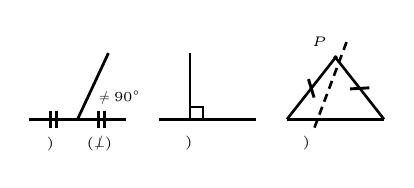
\begin{tikzpicture}[scale=0.56, every node/.style={font=\scriptsize, text=black}]
        % Trap 1: Slanted median (no 90)
        \begin{scope}[shift={(0,0)}]
          \draw[black, line width=1.0pt, tk2] (0,0)--(1.1,0); \draw[black, line width=1.0pt, tk2] (1.1,0)--(2.2,0);
          \draw[black, line width=1.0pt] (1.1,0)--(1.8,1.5);
          \node[font=\tiny, anchor=west] at (1.38,0.48) {$\neq 90^\circ$};
          \node[font=\tiny] at (1.1,-0.55) {១) ទ្រេត ($\not\perp$)};
        \end{scope}
        % Trap 2: Off-center perp (HB != HC)
        \begin{scope}[shift={(2.95,0)}]
          \coordinate (t2b) at (0,0); \coordinate (t2h) at (0.7,0); \coordinate (t2c) at (2.2,0); \coordinate (t2p) at (0.7,1.5);
          \draw[black, line width=1.0pt] (t2b)--(t2c); \draw[black, line width=1.0pt] (t2h)--(t2p);
          \pic[draw=black, line width=0.7pt, angle radius=1.6mm]{right angle=t2c--t2h--t2p};
          \node[font=\tiny] at (1.1,-0.55) {២) ខុសកណ្ដាល};
        \end{scope}
        % Trap 3: 1-point P trap
        \begin{scope}[shift={(5.85,0)}]
          \coordinate (g) at (0,0); \coordinate (h) at (2.2,0); \coordinate (p) at (1.1,1.4);
          \draw[black, line width=1.0pt] (g)--(h);
          \draw[black, line width=0.95pt, tkslash] (p)--(g); \draw[black, line width=0.95pt, tkslash] (p)--(h);
          \draw[black, densely dashed, line width=0.95pt] (1.35,1.75)--(0.60,-0.25);
          \fill[black] (p) circle (1.4pt) node[above left=0.5pt, font=\tiny] {$P$};
          \node[font=\tiny] at (1.1,-0.55) {៣) មានតែ ១ ចំណុច};
        \end{scope}
      \end{tikzpicture}
      \par\vspace{1.5pt}\fontsize{7.4pt}{10.4pt}\selectfont
      ខ្វះ $90^\circ$, ខ្វះ $IB=IC$, ឬស្មើចម្ងាយតែ \textbf{១ ចំណុច} ($PG=PH$ គ្មាន $2$ ចំណុច) $\Rightarrow$ \textbf{មិនមែន}មេដ្យាទ័រទេ!
    \end{tcolorbox}
  \end{minipage}
\end{tcolorbox}

\clearpage

% ============================================================================
% ទំព័រទី ៥៖ កាតវិនិច្ឆ័យរហ័ស ៦០–៩០ វិនាទី "កាត A–D" & ចម្លើយគ្រូ — E5 Evaluate
% ============================================================================
\pagebanner{សម្ភារៈទី ៥៖ កាតវិនិច្ឆ័យរហ័ស «កាត \enbf{A--D}» \enbf{(60--90} វិនាទី\enbf{) \&} ចម្លើយគ្រូ}{ទំព័រ ៥/៦ \en{-- E5 Evaluate}}

{\fontsize{8.5pt}{12pt}\selectfont
\textbf{វិធីលេងក្នុងថ្នាក់៖} គ្រូលើកកាតម្ដងមួយ $\rightarrow$ សិស្សផ្ទៀងសោភ្លោះ ($IB=IC$ \en{+} $90^\circ$) $\rightarrow$ លើក \textbf{មេដៃឡើង (ពិត \ding{51})} ឬ \textbf{ខ្វែងដៃ (ខុស/អន្ទាក់ \ding{55})} + ម្រាម \en{1--3}។}

\vspace{4pt}

% --- ជួរទី ១៖ កាត A & កាត B ---
\noindent
\begin{tcolorbox}[
  enhanced, sharp corners, colback=white, colframe=white,
  borderline={1.0pt}{0pt}{black, dashed},
  width=9.25cm, equal height group=pbfoilrow1, nobeforeafter,
  boxsep=1pt, top=5pt, bottom=5pt, left=6pt, right=6pt
]
  \noindent\colorbox{black}{\textcolor{white}{\Large\textbf{\en{ A }}}}\hspace{0.25cm}{\fontsize{9.2pt}{12.5pt}\selectfont\textbf{កាត \en{A} ៖ សោភ្លោះទ្រេត ($\Delta\perp AB$ ត្រង់ $I$)}}\par\vspace{2pt}
  \begin{center}
  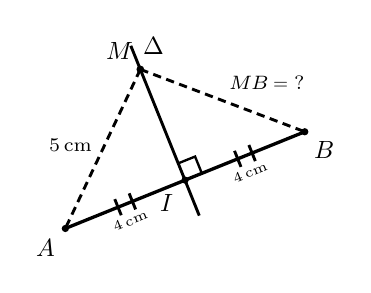
\begin{tikzpicture}[scale=0.82, every node/.style={font=\small, text=black}]
    % Tilted AB by 22 deg: I=(2.2, 1.0), A=(2.2-1.854, 1.0-0.749)=(0.346, 0.251), B=(4.054, 1.749)
    % Normal n=(-0.3746, 0.9272), M = I + 1.85*n = (1.507, 2.715)
    \coordinate (I) at (2.20, 1.00);
    \coordinate (A) at (0.346, 0.251);
    \coordinate (B) at (4.054, 1.749);
    \coordinate (M) at (1.507, 2.715);
    \coordinate (Dtop) at (1.36, 3.08);
    \coordinate (Dbot) at (2.42, 0.45);
    \draw[black, line width=1.2pt, tk2] (A) -- (I);
    \draw[black, line width=1.2pt, tk2] (I) -- (B);
    \draw[black, line width=1.05pt] (Dbot) -- (Dtop);
    \draw[black, densely dashed, line width=1.05pt] (M) -- (A);
    \draw[black, densely dashed, line width=1.05pt] (M) -- (B);
    \pic[draw=black, line width=0.85pt, angle radius=2.3mm]{right angle=B--I--M};
    \fill[black] (A) circle (1.6pt) node[below left=0pt] {$A$};
    \fill[black] (B) circle (1.6pt) node[below right=0pt] {$B$};
    \fill[black] (I) circle (1.6pt) node[below left=1.5pt] {$I$};
    \fill[black] (M) circle (1.7pt) node[above left=0pt] {$M$};
    \node[right=1pt] at (Dtop) {$\Delta$};
    \node[below=1pt, rotate=22, font=\tiny] at ($(A)!0.50!(I)$) {$4\unit{cm}$};
    \node[below=1pt, rotate=22, font=\tiny] at ($(I)!0.50!(B)$) {$4\unit{cm}$};
    \node[left=1pt, font=\scriptsize] at ($(M)!0.48!(A)$) {$5\unit{cm}$};
    \node[above right=0pt, font=\scriptsize] at ($(M)!0.48!(B)$) {$MB=?$};
  \end{tikzpicture}
  \end{center}
  {\centering\fontsize{8.0pt}{11pt}\selectfont $\Delta\perp AB$ ត្រង់ $I$ ($90^\circ$), $IA=IB=4\unit{cm}$, $M\in\Delta$, $MA=5\unit{cm}$~។\par}
  \vfill
  \begin{tcolorbox}[enhanced, sharp corners, colback=panelgray, colframe=black, boxrule=0.8pt, boxsep=1pt, top=4pt, bottom=4pt, left=5pt, right=5pt]
    \centering\fontsize{9.0pt}{12.5pt}\selectfont
    \textbf{សំណួរ៖} តើគេទាញបាន $MB = 5\unit{cm}$ ត្រឹមត្រូវឬទេ?\\[2pt]
    \chkbox\ មេដៃឡើង (\ding{51} ពិត) \hspace{0.4cm} \chkbox\ ខ្វែងដៃ (\ding{55} ខុស)
  \end{tcolorbox}
\end{tcolorbox}%
\hfill
\begin{tcolorbox}[
  enhanced, sharp corners, colback=white, colframe=white,
  borderline={1.0pt}{0pt}{black, dashed},
  width=9.25cm, equal height group=pbfoilrow1, nobeforeafter,
  boxsep=1pt, top=5pt, bottom=5pt, left=6pt, right=6pt
]
  \noindent\colorbox{black}{\textcolor{white}{\Large\textbf{\en{ B }}}}\hspace{0.25cm}{\fontsize{9.2pt}{12.5pt}\selectfont\textbf{កាត \en{B} ៖ អន្ទាក់មេដ្យានទ្រេត ($65^\circ$)}}\par\vspace{2pt}
  \begin{center}
  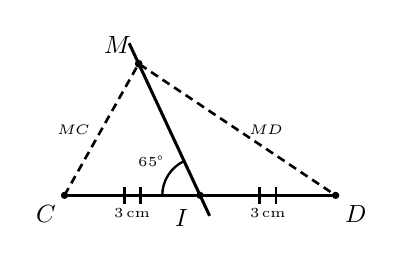
\begin{tikzpicture}[scale=0.82, every node/.style={font=\small, text=black}]
    % Segment CD horizontal: C=(0,0), D=(4.2,0), I=(2.1,0), slanted median at 65 deg from IC: angle 115 deg from ID? Wait: angle MIC=65 deg -> M is above-left of I: (-cos65, sin65)
    \coordinate (C) at (0, 0);
    \coordinate (D) at (4.20, 0);
    \coordinate (I) at (2.10, 0);
    \coordinate (M) at ($(I)+(115:2.25)$);
    \draw[black, line width=1.2pt, tk2] (C) -- (I);
    \draw[black, line width=1.2pt, tk2] (I) -- (D);
    \draw[black, line width=1.1pt] ($(I)+(-65:0.35)$) -- ($(I)+(115:2.60)$);
    \draw[black, densely dashed, line width=0.95pt] (C) -- (M) -- (D);
    \pic[draw=black, line width=0.85pt, angle radius=4.8mm]{angle=M--I--C};
    \node[font=\tiny] at ($(I)+(145:0.92)$) {$65^\circ$};
    \fill[black] (C) circle (1.6pt) node[below left=0pt] {$C$};
    \fill[black] (D) circle (1.6pt) node[below right=0pt] {$D$};
    \fill[black] (I) circle (1.6pt) node[below left=1.5pt] {$I$};
    \fill[black] (M) circle (1.7pt) node[above left=0pt] {$M$};
    \node[below=1pt, font=\tiny] at (1.05, 0) {$3\unit{cm}$};
    \node[below=1pt, font=\tiny] at (3.15, 0) {$3\unit{cm}$};
    \node[left=1pt, font=\tiny] at ($(C)!0.50!(M)$) {$MC$};
    \node[right=1pt, font=\tiny] at ($(D)!0.50!(M)$) {$MD$};
  \end{tikzpicture}
  \end{center}
  {\centering\fontsize{8.0pt}{11pt}\selectfont $IC=ID=3\unit{cm}$ តែបន្ទាត់តាម $I$ ទ្រេតបង្កើតមុំ $\ang{MIC}=65^\circ$~។\par}
  \vfill
  \begin{tcolorbox}[enhanced, sharp corners, colback=panelgray, colframe=black, boxrule=0.8pt, boxsep=1pt, top=4pt, bottom=4pt, left=5pt, right=5pt]
    \centering\fontsize{9.0pt}{12.5pt}\selectfont
    \textbf{សំណួរ៖} គេអះអាងថា $MC = MD$ ត្រឹមត្រូវឬទេ?\\[2pt]
    \chkbox\ មេដៃឡើង (\ding{51} ពិត) \hspace{0.4cm} \chkbox\ ខ្វែងដៃ (\ding{55} ខុស)
  \end{tcolorbox}
\end{tcolorbox}

\vspace{6pt}

% --- ជួរទី ២៖ កាត C & កាត D ---
\noindent
\begin{tcolorbox}[
  enhanced, sharp corners, colback=white, colframe=white,
  borderline={1.0pt}{0pt}{black, dashed},
  width=9.25cm, equal height group=pbfoilrow2, nobeforeafter,
  boxsep=1pt, top=5pt, bottom=5pt, left=6pt, right=6pt
]
  \noindent\colorbox{black}{\textcolor{white}{\Large\textbf{\en{ C }}}}\hspace{0.25cm}{\fontsize{9.2pt}{12.5pt}\selectfont\textbf{កាត \en{C} ៖ អន្ទាក់កែងខុសកណ្ដាល ($HE=2 \neq HF=5$)}}\par\vspace{2pt}
  \begin{center}
  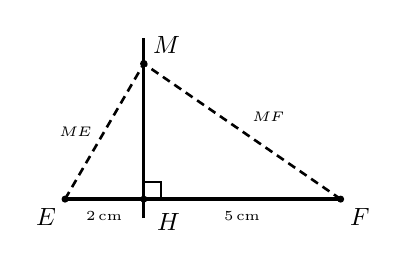
\begin{tikzpicture}[scale=0.80, every node/.style={font=\small, text=black}]
    % EF: E=(0,0), H=(1.25,0), F=(4.375,0) [exact 2:5 ratio!], M=(1.25, 2.25)
    \coordinate (E) at (0, 0);
    \coordinate (H) at (1.25, 0);
    \coordinate (F) at (4.375, 0);
    \coordinate (M) at (1.25, 2.15);
    \draw[black, line width=1.2pt] (E) -- (F);
    \draw[black, line width=1.1pt] (1.25, -0.30) -- (1.25, 2.55);
    \draw[black, densely dashed, line width=0.95pt] (E) -- (M) -- (F);
    \pic[draw=black, line width=0.85pt, angle radius=2.2mm]{right angle=F--H--M};
    \fill[black] (E) circle (1.6pt) node[below left=0pt] {$E$};
    \fill[black] (H) circle (1.6pt) node[below right=1.5pt] {$H$};
    \fill[black] (F) circle (1.6pt) node[below right=0pt] {$F$};
    \fill[black] (M) circle (1.7pt) node[above right=0pt] {$M$};
    \node[below=1pt, font=\tiny] at (0.625, 0) {$2\unit{cm}$};
    \node[below=1pt, font=\tiny] at (2.8125, 0) {$5\unit{cm}$};
    \node[left=1pt, font=\tiny] at ($(E)!0.50!(M)$) {$ME$};
    \node[above right=0pt, font=\tiny] at ($(F)!0.50!(M)$) {$MF$};
  \end{tikzpicture}
  \end{center}
  {\centering\fontsize{8.0pt}{11pt}\selectfont បន្ទាត់កែង $EF$ ត្រង់ $H$ ($90^\circ$) ដោយ $HE=2\unit{cm}$ និង $HF=5\unit{cm}$~។\par}
  \vfill
  \begin{tcolorbox}[enhanced, sharp corners, colback=panelgray, colframe=black, boxrule=0.8pt, boxsep=1pt, top=4pt, bottom=4pt, left=5pt, right=5pt]
    \centering\fontsize{9.0pt}{12.5pt}\selectfont
    \textbf{សំណួរ៖} គេអះអាងថា $ME = MF$ ត្រឹមត្រូវឬទេ?\\[2pt]
    \chkbox\ មេដៃឡើង (\ding{51} ពិត) \hspace{0.4cm} \chkbox\ ខ្វែងដៃ (\ding{55} ខុស)
  \end{tcolorbox}
\end{tcolorbox}%
\hfill
\begin{tcolorbox}[
  enhanced, sharp corners, colback=white, colframe=white,
  borderline={1.0pt}{0pt}{black, dashed},
  width=9.25cm, equal height group=pbfoilrow2, nobeforeafter,
  boxsep=1pt, top=5pt, bottom=5pt, left=6pt, right=6pt
]
  \noindent\colorbox{black}{\textcolor{white}{\Large\textbf{\en{ D }}}}\hspace{0.25cm}{\fontsize{9.2pt}{12.5pt}\selectfont\textbf{កាត \en{D} ៖ អន្ទាក់ ១ ចំណុច ($PG=PH=5\unit{cm}$)}}\par\vspace{2pt}
  \begin{center}
  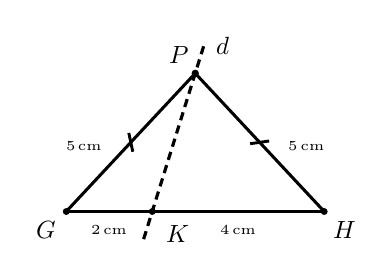
\begin{tikzpicture}[scale=0.78, every node/.style={font=\small, text=black}]
    % Isosceles triangle PGH: G=(0,0), H=(4.2,0) [scale 0.7 of 6cm], K at 2:4 -> x=1.40, P=(2.10, 2.40)
    \coordinate (G) at (0, 0);
    \coordinate (H) at (4.20, 0);
    \coordinate (K) at (1.40, 0);
    \coordinate (P) at (2.10, 2.25);
    \draw[black, line width=1.2pt] (G) -- (H);
    \draw[black, line width=1.1pt, tkslash] (P) -- (G);
    \draw[black, line width=1.1pt, tkslash] (P) -- (H);
    % Slanted line d passing through P and K (KG=2, KH=4)
    \draw[black, densely dashed, line width=1.15pt] ($(K)!-0.20!(P)$) -- ($(K)!1.22!(P)$);
    \fill[black] (G) circle (1.6pt) node[below left=0pt] {$G$};
    \fill[black] (H) circle (1.6pt) node[below right=0pt] {$H$};
    \fill[black] (K) circle (1.6pt) node[below right=1.5pt] {$K$};
    \fill[black] (P) circle (1.7pt) node[above left=0pt] {$P$};
    \node[right=1pt] at ($(K)!1.20!(P)$) {$d$};
    \node[above left=0.5pt, font=\tiny] at ($(G)!0.36!(P)$) {$5\unit{cm}$};
    \node[above right=0.5pt, font=\tiny] at ($(H)!0.36!(P)$) {$5\unit{cm}$};
    \node[below=1.5pt, font=\tiny] at (0.70, 0) {$2\unit{cm}$};
    \node[below=1.5pt, font=\tiny] at (2.80, 0) {$4\unit{cm}$};
  \end{tikzpicture}
  \end{center}
  {\centering\fontsize{8.0pt}{11pt}\selectfont $PG=PH=5\unit{cm}$ និងបន្ទាត់ទ្រេត $d$ កាត់តាម $P$ និង $K$ ($KG=2, KH=4$)~។\par}
  \vfill
  \begin{tcolorbox}[enhanced, sharp corners, colback=panelgray, colframe=black, boxrule=0.8pt, boxsep=1pt, top=4pt, bottom=4pt, left=5pt, right=5pt]
    \centering\fontsize{9.0pt}{12.5pt}\selectfont
    \textbf{សំណួរ៖} គេថាបន្ទាត់ $d$ ជាមេដ្យាទ័រនៃ $GH$ ត្រូវឬខុស?\\[2pt]
    \chkbox\ មេដៃឡើង (\ding{51} ពិត) \hspace{0.4cm} \chkbox\ ខ្វែងដៃ (\ding{55} ខុស)
  \end{tcolorbox}
\end{tcolorbox}

\vspace{6pt}

% --- ខ្សែកាត់ & បន្ទះចម្លើយសម្រាប់គ្រូ ---
\noindent\scissors\ \dotfill\ \textbf{កាត់ទុកសម្រាប់គ្រូ (\en{Teacher Mini Answer \& Remediation Key})} \dotfill\ \scissors

\vspace{4pt}
\begin{tcolorbox}[
  enhanced, sharp corners, colback=panelgray, colframe=black,
  boxrule=1.0pt, boxsep=1pt, top=4pt, bottom=4pt, left=5pt, right=5pt
]
  \fontsize{7.7pt}{10.8pt}\selectfont
  \renewcommand{\arraystretch}{1.10}
  \begin{tabular}{|L{4.25cm}|L{4.15cm}|L{4.15cm}|L{4.45cm}|}
    \hline
    \cellcolor{headgray}\textbf{កាត \en{A} ៖ មេដៃឡើង (\ding{51})} &
    \cellcolor{headgray}\textbf{កាត \en{B} ៖ ខ្វែងដៃ (\ding{55})} &
    \cellcolor{headgray}\textbf{កាត \en{C} ៖ ខ្វែងដៃ (\ding{55})} &
    \cellcolor{headgray}\textbf{កាត \en{D} ៖ ខ្វែងដៃ (\ding{55})} \\ \hline
    \textbf{ពិត!} មានសោភ្លោះពេញលេញ៖ $IA=IB=4\unit{cm}$ (\cnum{1}) និង $\Delta\perp AB$ ត្រង់ $I$ (\cnum{2}) $\Rightarrow MB=MA=5\unit{cm}$ (\cnum{4}) ទោះរូបទ្រេតក៏ដោយ។ &
    \textbf{អន្ទាក់មេដ្យានទ្រេត!} មាន $IC=ID=3\unit{cm}$ តែខ្វះសោ $90^\circ$ ($\ang{MIC}=65^\circ \neq 90^\circ$) $\Rightarrow MC\neq MD$។ &
    \textbf{អន្ទាក់កែងខុសកណ្ដាល!} មានមុំ $90^\circ$ តែខ្វះចំណុចកណ្ដាល ($HE=2 \neq HF=5$) $\Rightarrow ME\neq MF$។ &
    \textbf{អន្ទាក់ ១ ចំណុច!} មានតែ $P$ មួយ ($PG=PH=5$) មិនកំណត់ $\Delta$ ទេ ហើយ $KG=2\neq KH=4, d\not\perp GH$! ត្រូវការ \textbf{២ ចំណុច}។ \\ \hline
  \end{tabular}
  \par\vspace{2.5pt}
  \textbf{ត្រួតទំនុកចិត្ត (ម្រាម ១\en{--}៣)៖} ១ ម្រាម = ពិនិត្យសោភ្លោះ ($IB=IC$ \en{+} $90^\circ$) ជាមួយដៃគូ \hspace{0.15cm}\en{|}\hspace{0.15cm} ២ ម្រាម = ផ្ទៀងធនាគារ \cnum{1}--\cnum{5} \hspace{0.15cm}\en{|}\hspace{0.15cm} ៣ ម្រាម = ច្បាស់ ១០០\%
\end{tcolorbox}

\clearpage

% ============================================================================
% ទំព័រទី ៦៖ ប័ណ្ណកិច្ចការផ្ទះ ជំហានទី ៥ — ៤ ប័ណ្ណក្នុង ១ ទំព័រ A4 (4-up: HW #1, #3, #5)
% ============================================================================
\pagebanner{សម្ភារៈទី ៦៖ ប័ណ្ណកិច្ចការផ្ទះ ជំហានទី ៥ \enbf{--} ៤ ប័ណ្ណក្នុង ១ ទំព័រ \enbf{A4}}{ទំព័រ ៦/៦ \en{--} ជំហានទី ៥ (កាត់ ៤ ប័ណ្ណ \scissors)}

% ម៉ាក្រូប័ណ្ណកិច្ចការផ្ទះ ៤-up (ផ្ទៀង ១០០% នឹងលំហាត់ទី ១, ទី ៣, និងទី ៥ ទំព័រ ១៦៤)
\newcommand{\hwslipFourPB}[1]{%
\begin{tcolorbox}[
  enhanced, sharp corners, colback=white, colframe=white,
  borderline={0.95pt}{0pt}{black, dashed},
  width=9.25cm, equal height group=hwquadPB, nobeforeafter,
  boxsep=1pt, top=2.5pt, bottom=2.5pt, left=4pt, right=4pt
]
  \begin{tcolorbox}[
    enhanced, sharp corners, colback=headgray, colframe=black,
    boxrule=0.7pt, boxsep=1pt, top=1.5pt, bottom=1.5pt, left=4pt, right=4pt, after skip=2.5pt
  ]
    \fontsize{7.2pt}{9.8pt}\selectfont
    \textbf{\scissors\ កិច្ចការផ្ទះ (#1) \en{|} ២.១ មេដ្យាទ័រនៃអង្កត់} \hfill \textbf{អង្គារ ០១/១២/២៦}\\[1pt]
    ឈ្មោះ៖ $\underline{\hspace{4.0cm}}$ \hspace{0.2cm} ថ្នាក់៖ $\underline{\hspace{1.0cm}}$
  \end{tcolorbox}

  % --- លំហាត់ទី ១ (សៀវភៅទំព័រ ១៦៤) ---
  \noindent
  \begin{minipage}[c]{5.25cm}
    \fontsize{6.95pt}{9.6pt}\selectfont
    \textbf{លំហាត់ទី ១ (ទំ.១៦៤)៖} គេឱ្យ $\tri{ABC}\cg\tri{DEF}$ ដោយ $BC=(2x+30)\unit{cm}$ និង $EF=(5x-90)\unit{cm}$~។ គណនា $BC$~។\\
    {\fontsize{6.4pt}{8.9pt}\selectfont\textit{តម្រុយ៖} ជ្រុងត្រូវគ្នា $BC=EF \Rightarrow x=\underline{\hspace{0.45cm}} \Rightarrow BC=\underline{\hspace{0.55cm}}\unit{cm}$}
  \end{minipage}\hfill
  \begin{minipage}[c]{3.35cm}
    \centering
    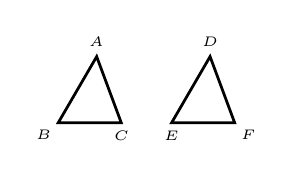
\begin{tikzpicture}[scale=0.40, every node/.style={font=\tiny, text=black}]
      \coordinate (B) at (0,0); \coordinate (C) at (2.0,0); \coordinate (A) at (1.22,2.1);
      \draw[black, line width=1.0pt] (A)--(B)--(C)--cycle;
      \node[above=0pt] at (A) {$A$}; \node[below left=-1pt] at (B) {$B$}; \node[below=-0.5pt] at (C) {$C$};
      \coordinate (E) at (3.6,0); \coordinate (F) at (5.6,0); \coordinate (D) at (4.82,2.1);
      \draw[black, line width=1.0pt] (D)--(E)--(F)--cycle;
      \node[above=0pt] at (D) {$D$}; \node[below=-0.5pt] at (E) {$E$}; \node[below right=-1pt] at (F) {$F$};
    \end{tikzpicture}
  \end{minipage}

  \vspace{2.5pt}\hrule height 0.45pt\vspace{2.5pt}

  % --- លំហាត់ទី ៣ (សៀវភៅទំព័រ ១៦៤ + បំបែក ∆MTO, ∆MBA) ---
  \noindent
  \begin{minipage}[c]{5.05cm}
    \fontsize{6.95pt}{9.6pt}\selectfont
    \textbf{លំហាត់ទី ៣ (ទំ.១៦៤)៖} គេឱ្យ $MT=MB$ និង $MA=MO$~។ បង្ហាញថា $\tri{MTO}\cg\tri{MBA}$~។\\
    {\fontsize{6.4pt}{8.9pt}\selectfont\textit{ប្រយ័ត្ន៖} រូបទំ.១៦៤ គ្មានគំនូសលើ $MT=MB$ ទេ — បំបែកត្រីកោណរកមុំរួម $\ang{M}$ (\textbf{ជ.ម.ជ})!}
  \end{minipage}\hfill
  \begin{minipage}[c]{3.55cm}
    \centering
    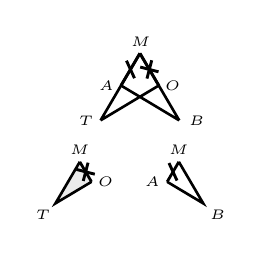
\begin{tikzpicture}[scale=0.37, every node/.style={font=\tiny, text=black}]
      % Book p. 164 Ex. #3 overlapped V + exploded silhouettes below
      \coordinate (M) at (1.35, 2.30);
      \coordinate (T) at (0.0, 0.0); \coordinate (B) at (2.70, 0.0);
      \coordinate (A) at ($(M)!0.48!(T)$); \coordinate (O) at ($(M)!0.48!(B)$);
      \draw[black, line width=0.95pt] (M)--(T) (M)--(B) (T)--(O) (A)--(B);
      \draw[black, line width=1.05pt, tkslash] (M)--(A);
      \draw[black, line width=1.05pt, tkcross] (M)--(O);
      \node[above=-1pt] at (M) {$M$}; \node[left=-1pt] at (A) {$A$}; \node[right=-1pt] at (O) {$O$};
      \node[left=0pt] at (T) {$T$}; \node[right=0pt] at (B) {$B$};
      % Exploded ∆MTO (left) and ∆MBA (right)
      \begin{scope}[shift={(-1.55, -2.85)}, scale=0.62]
        \coordinate (m1) at (1.35,2.30); \coordinate (t1) at (0,0); \coordinate (o1) at ($(m1)!0.48!(2.70,0)$);
        \fill[panelgray] (m1)--(t1)--(o1)--cycle;
        \draw[black, line width=0.95pt] (m1)--(t1)--(o1);
        \draw[black, line width=1.0pt, tkcross] (m1)--(o1);
        \node[above=-1pt] at (m1) {$M$}; \node[below left=-1pt] at (t1) {$T$}; \node[right=-1pt] at (o1) {$O$};
      \end{scope}
      \begin{scope}[shift={(1.85, -2.85)}, scale=0.62]
        \coordinate (m2) at (1.35,2.30); \coordinate (b2) at (2.70,0); \coordinate (a2) at ($(m2)!0.48!(0,0)$);
        \fill[white] (m2)--(a2)--(b2)--cycle;
        \draw[black, line width=0.95pt] (m2)--(b2)--(a2);
        \draw[black, line width=1.0pt, tkslash] (m2)--(a2);
        \node[above=-1pt] at (m2) {$M$}; \node[left=-1pt] at (a2) {$A$}; \node[below right=-1pt] at (b2) {$B$};
      \end{scope}
    \end{tikzpicture}
  \end{minipage}

  \vspace{2.5pt}\hrule height 0.45pt\vspace{2.5pt}

  % --- លំហាត់ទី ៥ (សៀវភៅទំព័រ ១៦៤ + (ខ) បន្ថែមមេដ្យាទ័រ) ---
  \noindent
  \begin{minipage}[c]{5.05cm}
    \fontsize{6.95pt}{9.6pt}\selectfont
    \textbf{លំហាត់ទី ៥ (ទំ.១៦៤)៖} \textbf{(ក)} គេឱ្យ $AB\parallel CD$ និង $TR=TS$~។ បង្ហាញថា $\tri{ABT}\cg\tri{DCT}$~។ \textbf{(ខ) បន្ថែម៖} បើគូស $\Delta\perp RS$ ត្រង់ $T$ តើ $\Delta$ ជាមេដ្យាទ័រនៃ $RS$ ទេ? ($MR \stackrel{?}{=} MS$)
  \end{minipage}\hfill
  \begin{minipage}[c]{3.55cm}
    \centering
    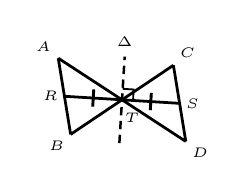
\begin{tikzpicture}[scale=0.45, every node/.style={font=\tiny, text=black}]
      % Book p. 164 Ex. #5 bowtie (NO polygon fills!)
      \coordinate (A) at (0, 2.35); \coordinate (B) at (0.35, 0.20);
      \coordinate (C) at (3.25, 2.15); \coordinate (D) at (3.60, 0.0);
      \coordinate (T) at (1.80, 1.175);
      \coordinate (R) at (0.175, 1.275);
      \coordinate (S) at (3.425, 1.075);
      \draw[black, line width=1.0pt] (A)--(B) (C)--(D) (A)--(D) (B)--(C);
      \draw[black, line width=1.0pt, tk1] (R)--(T);
      \draw[black, line width=1.0pt, tk1] (T)--(S);
      % Dashed Delta perp RS at T for part (ខ)
      \coordinate (Dbot) at ($(T)+(-0.075,-1.22)$);
      \coordinate (Dtop) at ($(T)+(0.075,1.22)$);
      \draw[black, densely dashed, line width=0.9pt] (Dbot) -- (Dtop);
      \pic[draw=black, line width=0.65pt, angle radius=1.4mm]{right angle=S--T--Dtop};
      \node[above left=-1pt] at (A) {$A$}; \node[below left=-1pt] at (B) {$B$};
      \node[above right=-1pt] at (C) {$C$}; \node[below right=-1pt] at (D) {$D$};
      \node[left=-1pt] at (R) {$R$}; \node[right=-1pt] at (S) {$S$};
      \node[fill=white, inner sep=0.25pt] at ($(T)+(-62:0.58)$) {$T$}; \node[above=0pt] at (Dtop) {$\Delta$};
    \end{tikzpicture}
  \end{minipage}

  \vspace{2.5pt}
  \begin{tcolorbox}[
    enhanced, sharp corners, colback=panelgray, colframe=black,
    boxrule=0.7pt, boxsep=1pt, top=2.5pt, bottom=2.5pt, left=4pt, right=4pt
  ]
    \fontsize{6.65pt}{9.4pt}\selectfont
    \textbf{ផ្ទៀងខ្លួនឯង (\en{Warrant \cnum{1}--\cnum{5}})៖}
    \chkbox\ បំបែកត្រីកោណ $\tri{MTO}, \tri{MBA}$ (លំ.៣) និង $\tri{ART}\cg\tri{DST} \to \tri{ABT}\cg\tri{DCT}$ (លំ.៥ក)!\\
    \chkbox\ ដាក់លេខហេតុផល \cnum{1}--\cnum{5} (៥ខ៖ $TR=TS$ [\cnum{1}] \en{+} $\Delta\perp RS$ [\cnum{2}] $\Rightarrow M\in\Delta \Rightarrow MR=MS$ [\cnum{4}])!
  \end{tcolorbox}
\end{tcolorbox}%
}

\noindent
\hwslipFourPB{ប័ណ្ណទី ១}\hfill\hwslipFourPB{ប័ណ្ណទី ២}

\vspace{6pt}
\noindent\scissors\ \dotfill\ \textbf{កាត់តាមស្នាមចុចចែកជា ៤ ប័ណ្ណ (\en{Cut Along Dashed Lines})} \dotfill\ \scissors
\vspace{6pt}

\noindent
\hwslipFourPB{ប័ណ្ណទី ៣}\hfill\hwslipFourPB{ប័ណ្ណទី ៤}

\end{document}
